\chapter{励磁}
\section{引言}
本章我们使用Bean于1962年提出的唯象磁化理论来讨论第II类超导体的磁化问题。如第一章指出的,对多数超导磁体应用所关注的磁场范围($>\sim 0.5T$),第II类超导体
处于混合态,即在超导态的“海”中还存在正常态的“岛”。当第II类超导体处于时变磁场或时变传输电流中时,这些岛中将产生耗散,体现为磁通跳跃(一种暂态现象)或交流损耗。
所谓的Bean临界态模型,以闭式表达式阐明了消除磁通跳跃和最小化交流损耗的必要条件。

如今,已经有了可以完全消除磁通跳跃的生产LTS线/缆的成熟方法。我们在本章将学习到,磁通跳跃在HTS中并不像在LTS中是那么重要。如果仅在消除磁通跳跃方面磁化是重要的,
那在HTS应用中可将其视为次要考虑问题。然而,由于磁化在LTS和HTS的交流损耗中也起到重要作用,所以我们用一章来研究它。交流损耗将在第七章有更详细的讨论。

\section{第II类超导体的Bean理论}
\subsection{无传输电流}
和很多成功的理论一样,Bean模型通过一些假设,可用简单的数学推导出闭式表达式,与实验结果取得了很好的一致性。在Bean模型中,超导体有最简单的几何结构——
$x$方向宽度为$2a$,$y$和$z$向无限长。磁场($H, B, M$)指向y向,而电流($I, J$)在z向流动。在Bean模型中,$J=J_c$(临界电流密度),并假定其不依赖于磁场和温度。

于是,磁场本构关系可以简化为下式:
\begin{equation}
  M=\frac{B}{\mu_0} -H
\end{equation}

根据Bean模型,磁感应强度B在硬超导体内的次表面内不为0,而是等于超导体的体平均$\mu_0 H_s$,$H_s$是超导体内的磁场。

%%图5.1
\begin{figure}[htbp]
  \centering
 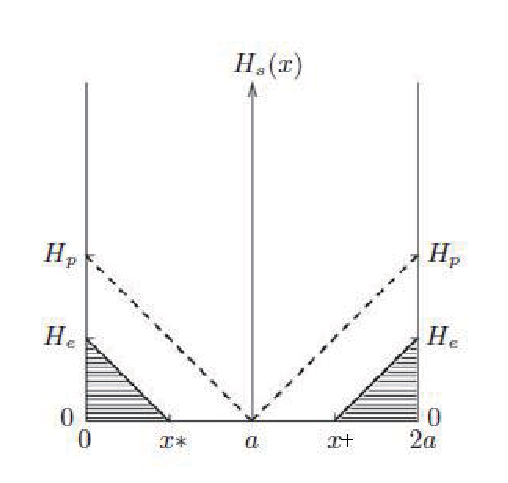
\includegraphics[scale=0.8]{chpt5/figs/fig5.1.eps}
  \caption{置于外磁场中的第II类超导体板}\label{fig:slabinfield}
\end{figure}
图\ref{fig:slabinfield}展示了第无限高($y$向)、无限深($z$向)、$2a$宽($x$向)第II类超导体板的。板此前未处于磁场中,外磁场$H_e$平行于板施加,将在板内产生$H_s(x)$。
根据安培定律$\nabla \times H = J=J_c$,我们可以得到超导体内的磁场$H_s(x)$:
%\begin{equation}
%  H_s(x)=
%  \begin{cases}
%           0, & \mbox{x*\le x \le x+ }  \\
%           H_e - J_c x, & \mbox{0\le x \le x* } \\
%           H_e + J_c (x-2a), & \mbox{x+ \le x \le 2a}
%   \end{cases}
%\end{equation}
注意到,$H_s(x)$的斜率等于$J_c$,当$J_c$大于0时(z向,朝向纸面外)大于0,$J_c$小于0时小于0。$x*$和$2a-x^+$给出磁场的穿透程度,表示为
\begin{equation}
  x*=\frac{H_e}{J_c}
\end{equation}

在$H_e=H_p\equiv J_c a$时,$x^*=x^+=a$,整个板处于临界态。$H_p$是所谓的穿透磁场,定义为
\begin{equation}
  H_p\equiv J_c a
\end{equation}

板内的平均磁感应强度由下式给出:
\begin{equation}
\begin{split}
\~{B}_s&=\frac{\mu_0}{2a}\int_{0}^{2a} H_s(x)dx \\
&=\frac{\mu_0}{2a}\times <\mbox{图5.1中的阴影面积}> \\
&=2\times \frac{\mu_0}{2a}\times \frac{H_e x^*}{2}=\frac{\mu_0 H_e^2}{2aJ_c}\\
&=\frac{\mu_0 H_e^2}{2H_p}
\end{split}
\end{equation}

根据定义$M=~{B}_s / \mu_0-H_e$,可得
\begin{equation}
  -M=H_e-\frac{H_e^2}{2H_p},(0\le H_e \le H_p)
\end{equation}

超导体是抗磁性的,-M是它的磁化强度。

随着外磁场的进一步增加,磁场将最终穿透整个板($H_e\ge H_p$),根据$~{B}_s=H_e-H_p/2$,有
\begin{equation}
  -M=\frac{1}{2}H_p=\frac{1}{2}J_c a, (H_e\ge H_p)
\end{equation}

图中的虚线磁化线对应$H_e=H_p$情况。
%5.2
\begin{figure}[htbp]
  \centering
 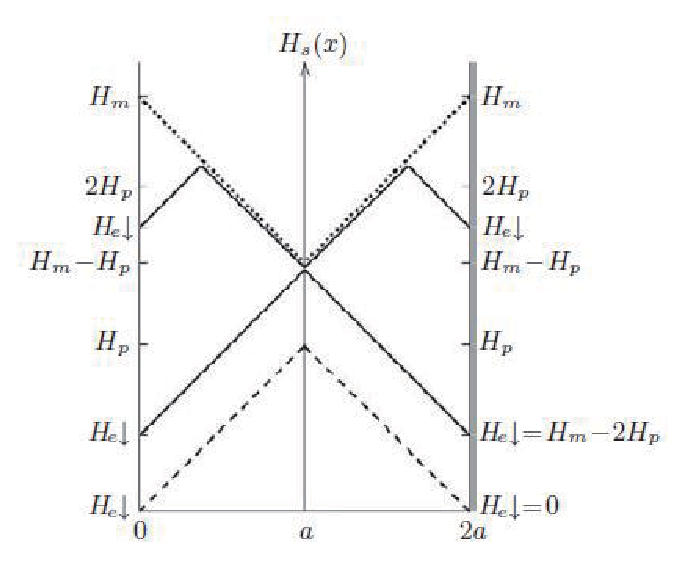
\includegraphics[scale=0.8]{chpt5/figs/fig5.2.eps}
  \caption{退场过程中的$H_s(x)$:$H_e\downarrow=H_m\rightarrow 0$}\label{fig:hreturn}
\end{figure}

图\ref{fig:hreturn}中的点线表示的是$H_s(x)$在$H_e=H_m>2H_p$时的情况。其中,$H_m$是外施磁场序列的最大值。

当$H_e$从$H_m$减至0的过程中,$H_s(x)$如图\ref{fig:hreturn}中的实线所示。当$H_e=H_m-2H_p$时,$-M$成为$-H_p /2$。
可以看到,外场从$H_m$到$H_e\downarrow=0$的退场过程中,$-M(H_e)$由下式给出
\begin{eqnarray}
% \nonumber % Remove numbering (before each equation)
  -M(H_e) =&\frac{1}{2}H_p-(H_m-H_e)+\frac{(H_m-H_e)^2}{4H_p}\\ \nonumber
                 & ,(H_e\downarrow=H_m\rightarrow H_m-2H_p) \\ \nonumber
  -M(H_e) =&-\frac{1}{2}H_p,\quad (H_e\downarrow=H_m-2H_p\rightarrow 0)
\end{eqnarray}

当外场施于“纯”板时,$-M$是$H_e$的二次函数。而在$H_e$退回0时,$-M(H_e)=-H_p /2$。“剩余”磁化如图\ref{fig:hreturn}中的虚划线所示。可知当置于外场中,
第II类超导体将会被磁化。剩余磁场不能通过外施磁场的方法去除。一种去除它的方法是加热超导体至临界温度$T_c$以上。
%5.3
\begin{figure}[htbp]
  \centering
 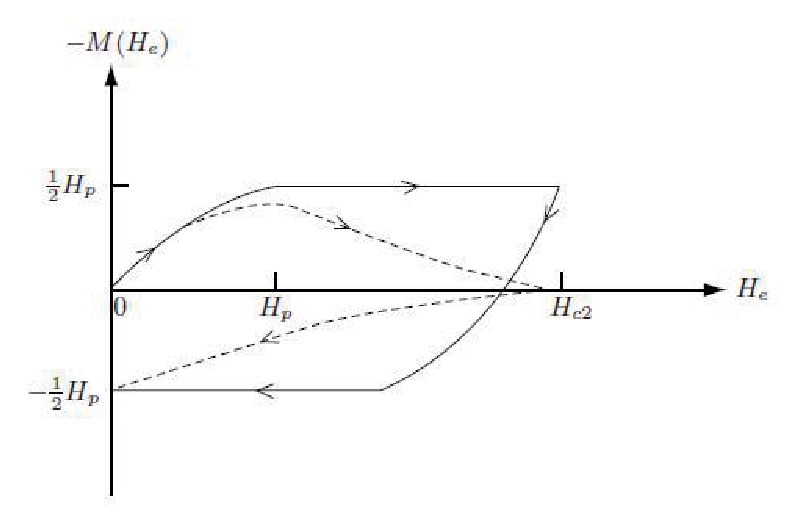
\includegraphics[scale=0.8]{chpt5/figs/fig5.3.eps}
  \caption{某硬超导体在外磁场($0\rightarrow H_{c2}\rightarrow 0$)下的磁化和磁场的关系。
  其中,实线表示$J_c=const$;虚线定性表示了电流随磁场下降的事实。}\label{fig:magvsh}
\end{figure}
图\ref{fig:magvsh}给出了完整的磁场从0增至$H_m=H_{c2}$又退回0的完整图像。其中,$H_{c2}$是超导体的上临界场。实线是基于由Bean的关于$J_c$不依赖磁场的假设
而导出的5.5-5.7式确定的。虚划线是对更接近实际情况的定性修正,反映了$J_c$随磁场衰减的事实,在$H_{c2}$时为0。注意到,磁化是有回滞的,在
$H_p<H_e<H_m-2H_p,\quad \Delta M=-M(H_e\uparrow)+M(H_e\downarrow)$范围内,磁场的幅值为$H_p=J_c a$。
于是,有时通过获得$J_e(H_e)$数据来做磁化的测量。
%5.4
\begin{figure}[htbp]
  \centering
 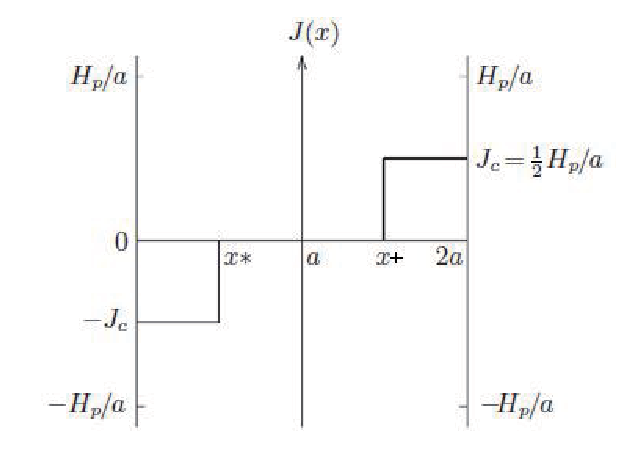
\includegraphics[scale=0.8]{chpt5/figs/fig5.4.eps}
  \caption{在图5.1给出的磁场$H_s(x)$下的$J(x)$}\label{fig:jtoh}
\end{figure}
图\ref{fig:jtoh}给出了在施加图\ref{fig:slabinfield}分布磁场下的板内电流分布。注意到$J_c=H_p /2a$。$y$向的单位长度净电流沿板的$z$向流动,由下式给出
\begin{equation}
  I=\int_{0}^{2a} J(x)dx=0
\end{equation}

\subsection{传输电流对励磁的效应}
当有传输电流$I_t$($y$向单位长度)在板中沿$+z$方向(流出纸面)时,我们看到在$x=2a$处磁场有一个$I_t/2$的增长,在$x=0$处有一个$I_t/2$的减少。

因为板内屏蔽电流是从每一个表面逐渐进入内部的,板内的场分布$H_s(x)$如图\ref{fig:hwithi}所示。图中的$x^*$和$x^+$由下式给出:
\begin{eqnarray}
% \nonumber % Remove numbering (before each equation)
  -\frac{1}{2}I_t + J_c x^* = 0 \\ \nonumber
  J_c(x^*-2a)+\frac{1}{2}I_t = 0 \\ \nonumber
  x^*=\frac{I_t}{2J_c}\quad \& \quad x^+ = 2a-\frac{I_t}{2J_c}
\end{eqnarray}

%%%%图5.5
\begin{figure}[htbp]
  \centering
 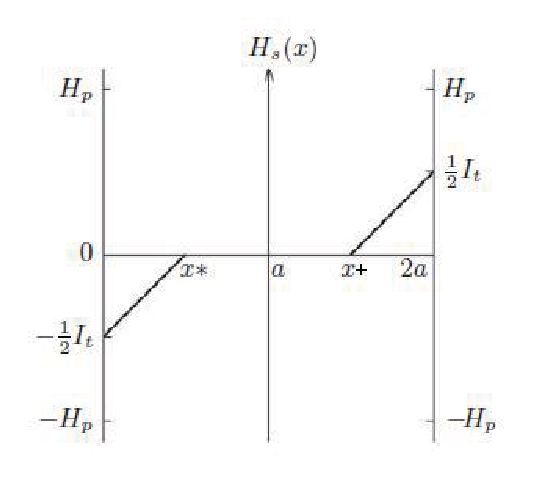
\includegraphics[scale=0.8]{chpt5/figs/fig5.5.eps}
  \caption{板内存在传输电流$I_t$时的磁场$H_s(x)$}\label{fig:hwithi}
\end{figure}

图5.6给出了板内的电流分布$J(x)$。沿着板宽度方向积分,我们可以得到板内的净电流就是$I_t$:
\begin{equation}
  I=\int_{0}^{2a}J(x)dx=J_c x^*+J_c(2a-x^+)=1/2 I_t +1/2 I_t=I_t
\end{equation}

\begin{figure}[htbp]
  \centering
 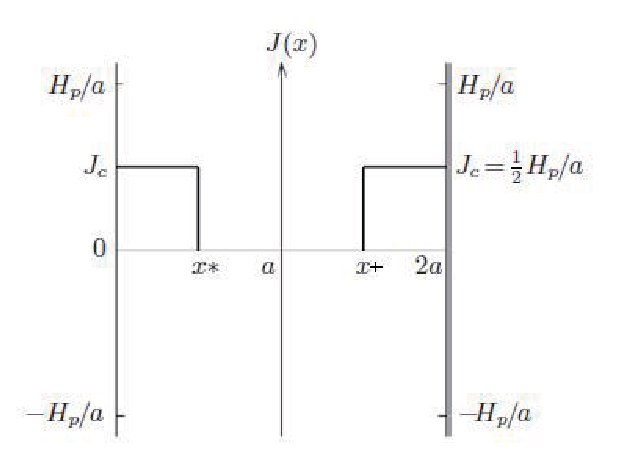
\includegraphics[scale=0.8]{chpt5/figs/fig5.6.eps}
  \caption{在图5.5给出的磁场$H_s(x)$下的$J(x)$}\label{fig:jtoh5.5}
\end{figure}

也即,板内的净电流就是外施电流。注意到,若外磁场$H_e\vec{i_y}$在$I_t$通入后施加,基本不会改变电流的分布(图5.5和5.6);但若外磁场
先于电流施加,则会出现不同的$H_s(x)$和$J(x)$。

\section{测量技术}
这里我们描述最经常使用的测量磁化的技术。图5.7指示了本项技术的关键组件:1)初级查找线圈;2)次级查找线圈;3)平衡分圧计。
图中未画出但也同等重要的是积分器,它将桥路输出电压$V_bg$转换为直接正比于$M(H_e)$的电压信号。测试样品置于初级查找线圈内,。
当初级查找线圈和次级查找线圈置于在两个线圈所占的空间内基本均匀的时变外磁场$H_e(t)$中,各查找线圈的端子上将出现感应
电压$V_{pc}(t)$和$V_{sc}(t)$:
\begin{eqnarray}
% \nonumber % Remove numbering (before each equation)
  V_{pt}(t) &=& \mu_0 N_{pc} A_{pc}\left[ \frac{dM}{dt}+(\frac{d\~{H}_e}{dt})_{pc}\right] \\ \nonumber
  V_{sc}(t) &=& \mu_0 N_{sc} A_{sc}\left( \frac{d\~{H}_e}{dt}\right)_{sc}
\end{eqnarray}

下标pc和sc分别表示初级线圈(primary coil)和次级线圈(second coil)。N是各线圈的匝数。A是耦合$H_e(t)$的每一匝线圈的有限面积。
$\~{H}_e$是磁场在各线圈内的空间平均值。

桥输出电压$V_bg$由下式给出:
\begin{equation}
  V_{bg}(t)=(k-1)V_{pt}(t)+kV_{sc}(t)
\end{equation}

其中,k是一个介于0-1的常数,表示分压计在初级线圈侧的分压系数(图5.7)。联立上两式,可得
\begin{equation}
  V_{bg}(t)=(k-1)\mu_0 N_{pc}A_{pc}\frac{dM}{dt}+(k-1)\mu_0 N_{pc}A_{pc}(\frac{d\~{H}_e}{dt})_{pc}+k\mu_0 N_{sc}A_{sc}(\frac{d\~{H}_e}{dt})_{sc}
\end{equation}

%%图5.7
\begin{figure}[htbp]
  \centering
 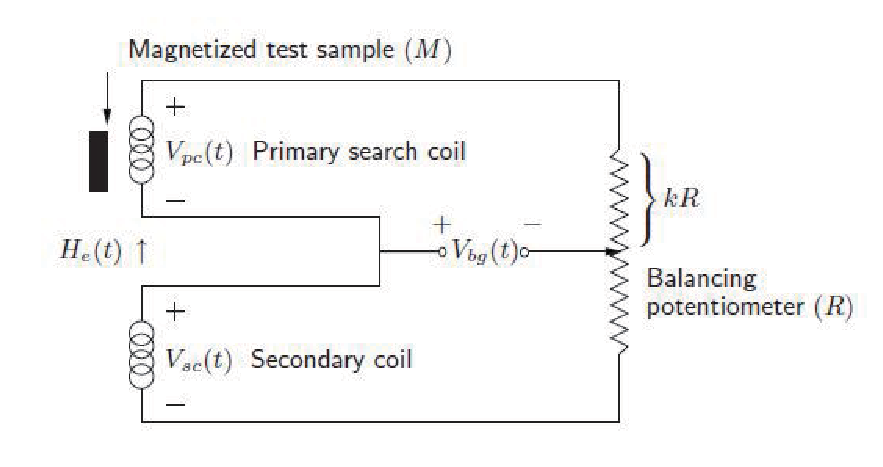
\includegraphics[scale=0.8]{chpt5/figs/fig5.7.eps}
  \caption{磁化测量原理图}\label{fig:magmeasure}
\end{figure}

通过调节分压系数k可以满足以下条件,令$V_{bg}(t)$正比于$dM/dt$:
\begin{eqnarray}
% \nonumber % Remove numbering (before each equation)
  &(k-1)\mu_0 N_{pc}A_{pc}(\frac{d\~{H}_e}{dt})_{pc}+k\mu_0 N_{sc}A_{sc}(\frac{d\~{H}_e}{dt})_{sc}=0 \\ \nonumber
  &V_{bg}(t)=(k-1)\mu_0 N_{pc}A_{pc}\frac{dM}{dt}
\end{eqnarray}

尽管实际上上式第一式所给的归零条件在很大范围内不是总能满足,但是第二式对多数情况都是很好的近似。
一般,$k$接近0.5。$V_bg{t}$馈入一个积分器,其输出正比于$M$。特别的,如果样品是“纯”的($M=0$),磁场
$H_e(t)$从0($t=0$)增($\uparrow$)至$H_e$($t=t_1$)时,我们有
\begin{equation}
  V_{mz}(H_e\uparrow)=\frac{1}{\tau_{it}}\int_{0}^{t_1}V_bg(t)dt=\frac{(k-1)\mu_0 N_{pc}A_{pc}}{\tau_{it}}M(H_e)
\end{equation}

式中,$\tau_{it}$是有效积分常数。如果$H_e>H_p$,此时有$M(H_e)=-H_p / 2=-J_c a / 2$,则上式简化为
\begin{equation}
    V_{mz}(H_e\uparrow>H_p)=-f_m \frac{(k-1)\mu_0 N_{pc}A_{pc}}{\tau_{it}}(\frac{J_c a}{2})
\end{equation}

因数$f_m$是磁性材料体积与样品总体积之比。之所以需要这个因数是因为待磁化测试的样品一般不全是由磁性材料组成。
比如多丝(层)导体,样品除了超导丝(层)外,还存在基底金属和其他非磁性材料。如果外场按$0\rightarrow H_m>H_p\rightarrow H_e\downarrow <H_m-2H_p$顺序,
我们有
\begin{equation}
    V_{mz}(H_e\downarrow<H_m-2H_p)=-f_m \frac{(k-1)\mu_0 N_{pc}A_{pc}}{\tau_{it}}(\frac{J_c a}{2})
\end{equation}

于是,$\Delta V_{mz}=V_{mz}(H_e>H_p)-V_{mz}(H_e\downarrow<H_m-2H_p)$正比于在$H_e$处磁化曲线的“宽度”:
\begin{equation}
    \Delta V_{mz}=-f_m \frac{(k-1)\mu_0 N_{pc}A_{pc}}{\tau_{it}} J_c a
\end{equation}

上式我们看出,$\Delta V_{mz}$是直接正比于$J_c$和$a$的。
%%图5.8
\begin{figure}[htbp]
  \centering
 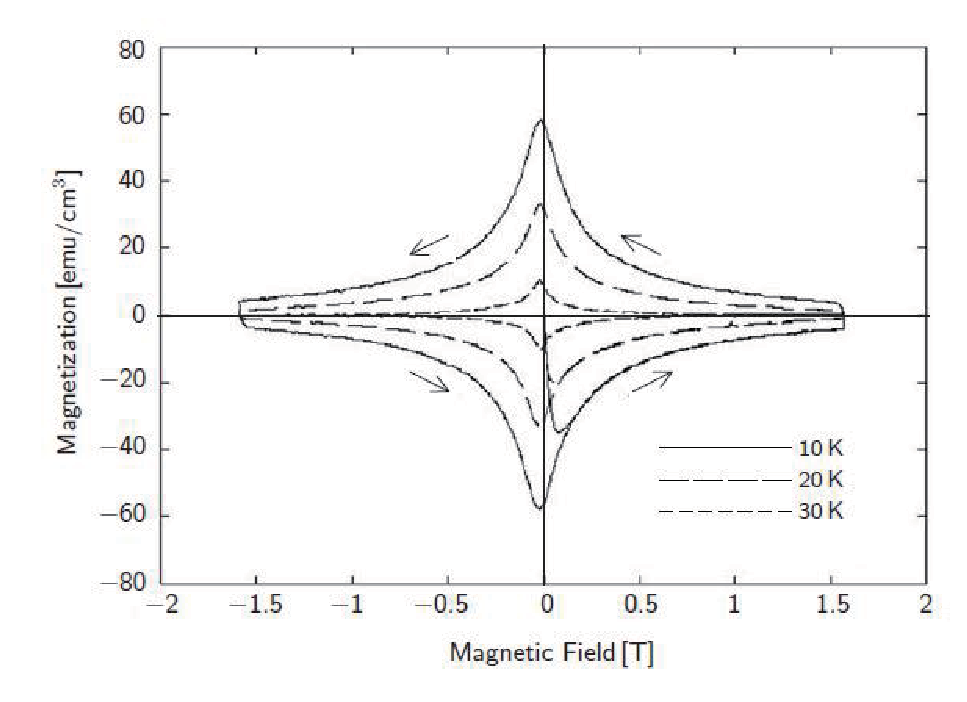
\includegraphics[scale=0.7]{chpt5/figs/fig5.8.eps}
  \caption{$MgB_2$在$10K,20K,30K$三种温度下的磁化和磁场关系}\label{fig:magvfield}
\end{figure}
图5.8给出的是$MgB_2$在10K,20K,30K时,磁场按$0\rightarrow 1.7T\rightarrow 0 \rightarrow -1.7T\rightarrow 0$完整施加时的磁化与磁场的关系。注意到,
和图5.3不同,本图中还有$+M(H_e)$。因为凸显在$x$轴上(磁场)并不偏斜,我们可以认为本测试中初次、二次线圈已得到很好的平衡。

磁化的回滞表明,$MgB_2$是第II类超导体,它的抗磁性在每一个图线的第一部分(磁场从0增至1.7T时)明显可见。

从Bean模型可知,$H_p=J_c a$,即磁化直接正比于$J_c$。然而,实际上$J_c$不仅是磁场还是温度的减函数。图5.8中明显可见对$J_c$和$T$的依赖。
图中的$M$的单位是$emu/cm^3$,不是SI单位。

\section{专题}
\subsection{讨论5.1:传输电流磁化}
正如本书最初所述,在传输电流存在条件下的励磁依赖于外场和传输电流施加的顺序。
这里我们考虑三种情况:A) 先加磁场后加传输电流; B) 先通电流后加磁场;C) 磁场和电流交替改变。

\textbf{A.  先加磁场后加传输电流}

图5.9给出了厚度为$2a$的Bean板在施加如下特定磁场-电流序列后内部磁场$H_s(x)$的特征。
\begin{enumerate}
	\item 起始,$H_{s1}(x)$,有$H_e=2.5H_p$,无传输电流——点线。
	\item 接下来,$H_{s2}(x)$,通过传输电流$I_t=J_c=I_c/2$后,施加恒定外场——实线。其中,$J_c a=H_p$。
	\item 最后,$H_{s3}(x)$,传输电流进一步增加到$2J_c a=I_c$后,磁场$H_e =2.5 H_p$,最终$H_{s3}(0)=1.5 H_p$
	以及$H_{s3}(2a)=3.5H_p$——虚线。
\end{enumerate}

$H_{s1}(x)$和$H_{s3}(x)$是很直接的。$H_{s2}(x)$由三个分段函数$H_{s2_1}(x),H_{s2_2}(x),H_{s2_3}(x)$组成:
\begin{align*}% page321 第1个
H_{s2_{1}}(x)&=2H_{p}+J_{c}x=2J_{c}a+J_{c}x\qquad&(0\leq x\leq x*)\\
H_{s2_{2}}(x)&=2.5H_{p}-J_{c}x=2.5J_{c}a-J_{c}x\quad&(x*\leq x\leq x+)\\
H_{s2_{3}}(s)&=H_{p}+J_{c}x=J_{c}a+J_{c}x\qquad&(x+\leq x\leq 2a)
\end{align*}
式中,$x*$和$x+$由$H_{s1}(x)$和$H_{s2}(x)$的两个拐点给出。也即,$H_{s1}(x*)=H_{s2_1}(x*)$,
$H_{s1}(x+)=H_{s2_3}(x+)$:$x*=0.25a$,$x+=0.75a$。
\begin{figure}[htbp]
	\centering
	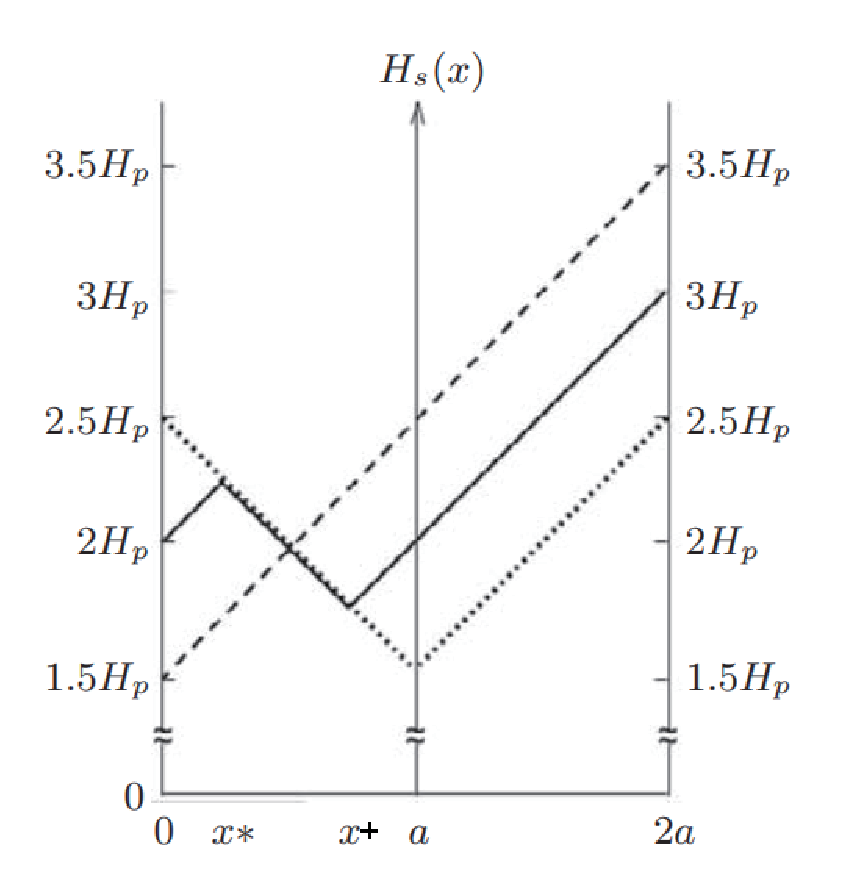
\includegraphics[scale=0.6]{chpt5/figs/fig5.9.eps}
	\caption{在$H_e=2.5H_p$下的磁场特征。首先,$I_t$=0(点线),然后$I_t=J_c a=I_c/2$(实线),最后$I_t=2J_c a=I_c$(虚线)。}
\end{figure}

图5.10给出了。。。。。

面积A1.。。。。。。

\begin{align*}
H_{s2_{1}}(x)&=(H_{e}-\frac{1}{2}I_{t})+J_{c}x\qquad&(0\leq x\leq x*)\\
H_{s2_{2}}(x)&=H_{e}-J_{c}x\qquad&(x*\leq x\leq x+)\\
H_{s2_{s}}(x)&=(H_{e}+\frac{1}{2}I_{t})+J_{c}(x-2a)\qquad&(x+\leq x\leq2a)
\end{align*}
我们解出$x*$和$x+$,确定$H_{s2_2}(x*)$和$H_{s2_2}(x+)$:
\begin{align*}
&H_{{s}2_{1}}(x*)=H_{s2_{2}}(x*)\\
&H_{e}-H_{p}i+J_{c}x*=H_{e}J_{c}x*\Rightarrow x*=\frac{H_{p}}{2J_{c}}i=\frac{1}{2}ai\\
&H_{s2_{2}}(x*)=H_{e}-\frac{1}{2}aJ_{c}i=H_{e}-\frac{1}{2}H_{p}i
\end{align*}
以及
\begin{align*}
H_{s2_{2}}(x+)&=H_{s2_{3}}(x+)\\
H_{e}-J_{c}x+&=H_{e}+H_{p}i+J_{c}(x^{+}-2a)\Rightarrow x^{+}=a(1-\frac{1}{2}i)\\
H_{s2_{2}}(x+)&=H_{e}-H_{p}+\frac{1}{2}H_{p}i
\end{align*}

\begin{figure}[htbp]
	\centering
	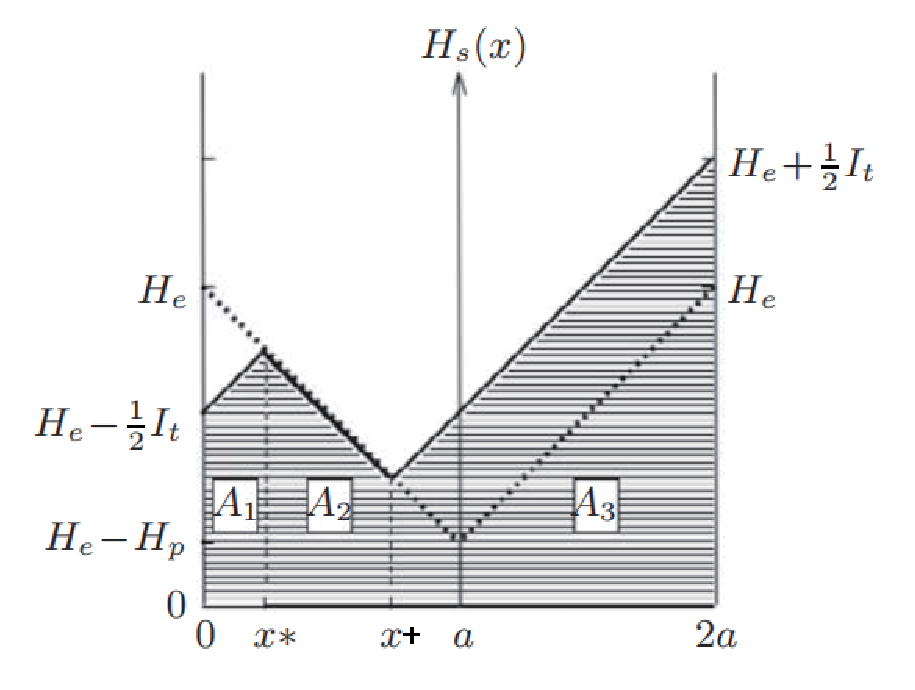
\includegraphics[scale=0.6]{chpt5/figs/fig5.10.eps}
	\caption{用于励磁计算的有传输电流(实线)的磁场的特征。竖直点线分开三个区域:$A_1, A_2$和$A_3$。}
\end{figure}

$M$正比于如图5.10所示的``阴影面积``大小,是三个部分面积$A_1, A2$及$A_3$之和。

各梯形的面积为它的``底边$\times$(高1+高2)/2``。
\begin{align*}% page323 第1个
A_{1}&=\frac{1}{2}x*[H_{s1}(0)+H_{s2}(x*)]=\frac{1}{4}ai[(H_{e}-H_{p}i)+(H_{e}-\frac{1}{2}H_{p}i)]\\
&=\frac{1}{4}ai(2H_{e}-\frac{3}{2}H_{p}i)  \\
&=a(\frac{1}{2}H_{e}i-\frac{3}{8}H_{P}i^{2})\\
A_{2}&=\frac{1}{2}(x^{+}-x*)[H_{s2}(x*)+H_{s2}(x^{+})]\\
&=\frac{1}{2}(a-ai)(H_{e}-\frac{1}{2}H_{p}i+H_{e}-H_{p}+\frac{1}{2}H_{p}i)\\
&=\frac{1}{2}a(-i)(2H_{e}-H_{p})\\
&=a(H_{e}-H_{e}i-\frac{1}{2}H_{p}+\frac{1}{2}H_{p}i)\\
A_{3}&=\frac{1}{2}(2a-x+)[H_{s2}(x+)+H_{s3}(2a)]\\
&=\frac{1}{2}(a+\frac{1}{2}ai)(H_{e}-H_{p}+\frac{1}{2}H_{p}i+H_{e}+H_{P}i)\\
&=a(1+\frac{1}{2}i)(H_{e}-\frac{1}{2}H_{p}+\frac{3}{4}H_{p}i)\\
&=a(H_{e}+\frac{1}{2}H_{e}i-\frac{1}{2}H_{p}-\frac{1}{4}H_{p}i+\frac{3}{4}H_{p}i+\frac{3}{8}H_{p}i^{2})
\end{align*}
组合这三个面积,我们可以计算出阴影面积:
\begin{align*}% page323 第4个
\text{Shaded\quad area}=&A_{1}+A_{2}+A_{3}\\
=&a(\frac{1}{2}H_{e}i-\frac{3}{8}H_{p}i^{2}+H_{e}-H_{e}i-\frac{1}{2}H_{p}+\frac{1}{2}H_{p}i\\
&+H_{e}+\frac{1}{2}H_{e}i-\frac{1}{2}H_{p}-\frac{1}{4}H_{P}i+\frac{3}{4}H_{P}i+\frac{3}{8}H_{p}i^{2})\\
=&a(2H_{e}-H_{p}+H_{p}i)
\end{align*}
一旦阴影面积已知,$M$可快速算出:
\begin{align*}% page323 第4个
-M(i)&=H_{e}-\frac{1}{2a}\times(Shaded\quad area)\\
&=H_{e}-H_{e}+\frac{1}{2}H_{p}-\frac{1}{2}H_{p}i\\
&=\frac{1}{2}H_{p}(1-i)\\
&=-M(0)f_{1}(i)
\end{align*}
式中,$f_1(i) = 1 − i$。$−M(i)$线性随$i$减小,当$i=1$时为零。 

\textbf{B. 先通电流后加磁场}

这里向板加外部磁场和传输电流顺序是反过来的。。。。。。。

在图4.11中,。。。。。

开始,$H_e=0$:
\begin{align*}% page324 第1个
I_{t}=\int_{0}^{2a}J(x)dx=J_{c}(0.5)+J_{c}(2a-1.5a)=J_{c}a
\end{align*}
接下来,$H_e=2H_p$:
\begin{align*}% page324 第2个
I_{t}=\int_{0}^{2a}J(x)dx=-J_{c}(0.5a)+J_{c}(2a-0.5a)=J_{c}a
\end{align*}
为了确定板内的励磁。。。。。。。
\begin{align*}
H_{s1}(x)&=(H_{e}-H_{p}i)-J_{c}x\qquad(0\leq \leq x*)\\
H_{s2}(x)&=(H_{e}+H_{p}i)+J_{c}(x-2a)\quad(x*\leq x leq  2a)
\end{align*}
因为,。。。。。。
\begin{align*}% page324 第5个
x*=a-ai=a(1-i)
\end{align*}

\begin{figure}[htbp]
	\centering
	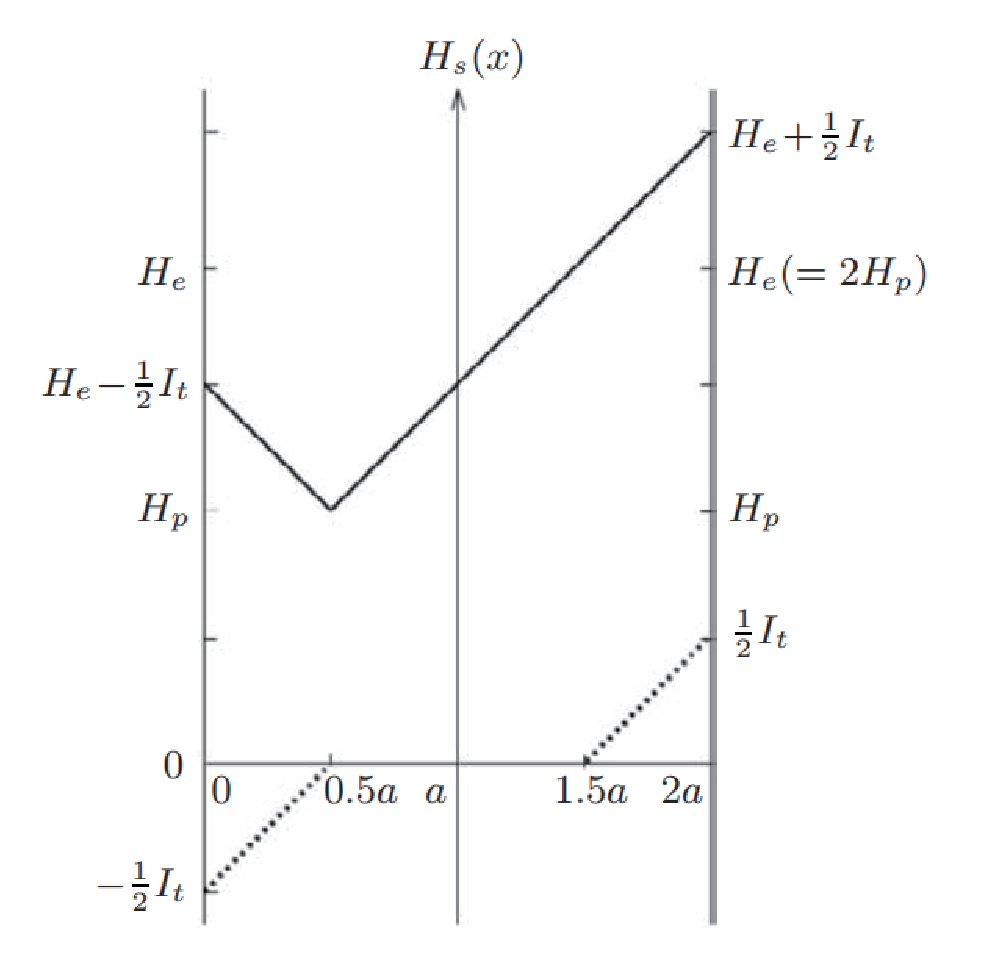
\includegraphics[scale=0.5]{chpt5/figs/fig5.11.eps}
	\caption{磁场特征,点线表示仅有电流,实现表示有磁场和电流。}
\end{figure}

确定了$x*$之后,我们可以计算$H_{s1}(x∗)$:
\begin{align*}% page325 第1个
H_{s1}(x*)=H_{e}-H_{p}i-J_{c}a(1-i)=J_{e}-H_{p}
\end{align*}
接下来我们可以计算阴影下的面积,即如图5.12中所示的由竖直线分开的A1和A2两部分之和:
\begin{align*}% page325 第2个
A_{1}&=\frac{1}{2}a(1-i)(H_{e}-H_{p}i+H_{e}-H_{p}\\
&=a(1-i)(H_{e}\frac{1}{2}H_{p}-\frac{1}{2}H_{p}i)\\
&=a(H_{e}-H_{e}i\frac{1}{2}H_{p}+\frac{1}{2}H_{p}i^{2})
A_{2}&=\frac{1}{2}(2a-a+ai)(H_{e}+H_{p}i+H_{e}-H_{P})\\\notag
&=a(1+i)(H_E-\frac{1}{2}H_{p}+\frac{1}{2}H_{p}i)\\\notag
&=a(H_{e}+H_{e}-\frac{1}{2}H_{p}+\frac{1}{2}H_{p}i^{2})
\end{align*}
\begin{align*}% page325 第4个
\text{Shaded\quad area}&=A_{1}+A_{2}\\
&=a(2H_{e}-H_{p}+H_{p}i^{2})
\end{align*}
计算了阴影面积后,我们有$M$:
\begin{subequations}
	\begin{align*}
-M(i)&=H_{e}-\frac{1}{2}(2H_{e}-H_{p}+H_{P}i^{2}\\\notag
&=\frac{1}{2}H_{p}(1-i^{2})\\
&=-M(0)f_{2}(i)
	\end{align*}
\end{subequations}
式中,$f_2(i) = 1 − i^2$。励磁时电流$i$的二次函数。

\begin{figure}[htbp]
	\centering
	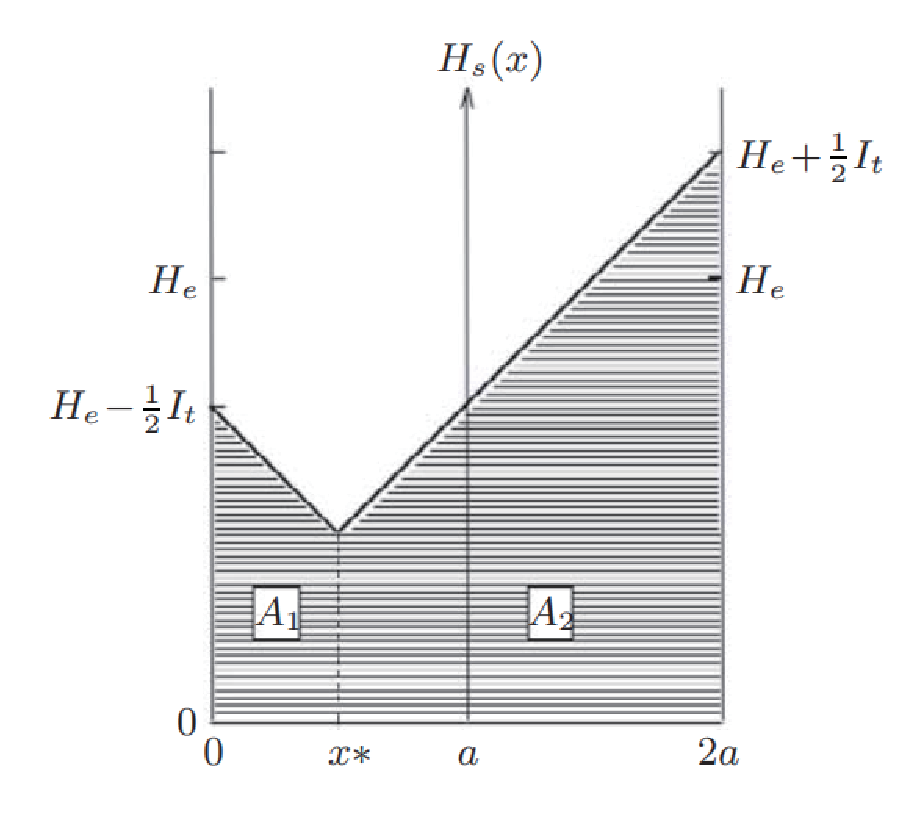
\includegraphics[scale=0.6]{chpt5/figs/fig5.12.eps}
	\caption{用以计算励磁的同时有传输电流和磁场的场特性磁场特征。竖直点线分出两个区域$A_1$和$A_2$。}
\end{figure}


\textbf{C. 磁场和电流交替改变}

最后,我们可以考虑按照以下序列施加磁场和传输电流时的$H_s(x)$和$−M(i)$。

\begin{enumerate}
	\item 开始
	\item 当
	\item 当
	\item 现在
	\item 再一次
\end{enumerate}

Figure 5.13 shows the field profile Hs(x) after Step 5, consisting of five piece-wise
solid lines, the second and third of which, useful to compute M(i), are given below.
\begin{align*}
H_{s2}(x)&=H_{e}+H_{p}i-J_{c}x\qquad(x*\leq x\leq a)\\
H_{s3}(x)&=H_{e}+H_{p}i+J_{c}(x-2a)\quad(a\leq x\leq a^{+})
\end{align*}
式中,$x∗$和$x$可由$H_{s2}(x∗)=H_{s3}(x)=H_e$解出。于是:
\begin{align*}
H_{s2}(x*)&=H_{e}\Rightarrow H_{e}+H_{p}i-J_{c}x*\\
x*&=\frac{H_{p}i}{J_{c}}=ai\\
H_{s3}(x+)&=H_{e}\Rightarrow H_{e}+H_{P}i+J_{c}(x^{+}-2a)\\
x^{+}&=2a-\frac{H_{p}}{J_{c}}i=2a-ai
\end{align*}

\begin{figure}[htbp]
	\centering
	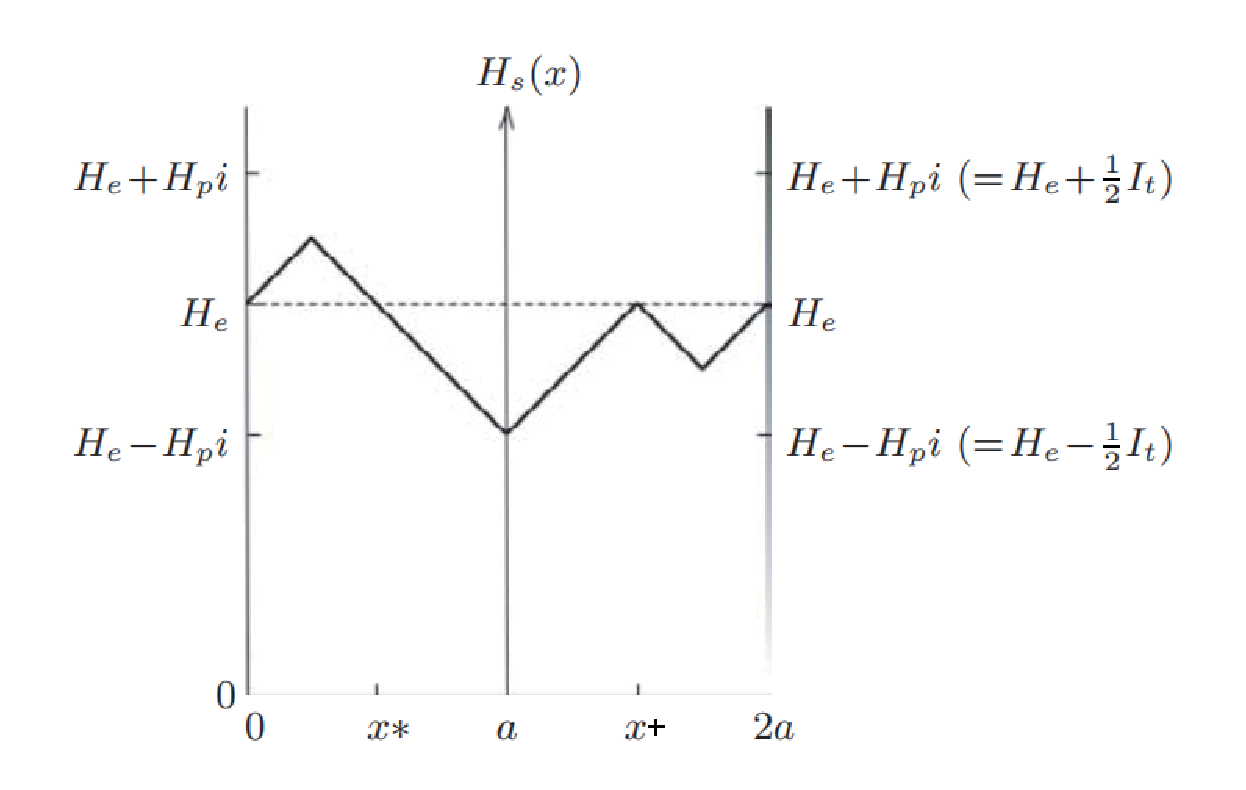
\includegraphics[scale=0.5]{chpt5/figs/fig5.13.eps}
	\caption{第五步之后的磁场特征。}
\end{figure}

The magnetization is computed from appropriate areas, shown in Fig. 5.14, in
which the slab is divided into four “white” areas, from left to right, designated A1
(rectangle), A2 (trapezoid), A3 (trapezoid), and A4 (rectangle minus “triangle”).
In the figure, “base” and “height” are given by:
\begin{align*}
\text{base}&=x+-x*=(2a-ai)-ai=(a(1-i)\\
\text{height}&=H_{e}-H_{s2}(a)=H_{e}-(H_{e}+H_{p}i-J_{c}a)\\
&=J_{c}a-J_{p}i=H_{p}(1-i)
\end{align*}
The two “dotted” areas in Fig. 5.14 are equal in magnitude but have “opposite”
signs, hence they cancel out when we perform the area integral. The sum of the
areas, A1, A2, A3, and A4, is given by:
\begin{align*}
\sum_{j=1}^{4}A_{j}&=2aH_{e}-\text{crossed\quad area}\\
crossed\quad area&=\frac{1}{2}(base)\times(height)\\
\sum_{j=1}^{4}A_{j}&=2aH_{e}-\frac{1}{2}2a(1-i)H_{p}(1-i)\\
&=2aH_{e}-aH_{p}(1-i)^{2}
\end{align*}
于是,磁化$−M(i)$可如下给出:
\begin{align*}% page327 第6个
-M(i)&=H_{e}-\frac{1}{2a}[2aH_{e}-a \grave{}H_{p}(1-i)^{2}]\\
&=\frac{1}{2}H_{p}(1-i)^{2}
\end{align*}
\begin{subequations}
	\begin{align*}
-M(i)=&-M(0)(1-i)^{2}\\
=&-M(0)f_{3}(i)
	\end{align*}
\end{subequations}
式中,$f_3(i) = (1 − i)^2$。

\begin{figure}[htbp]
	\centering
	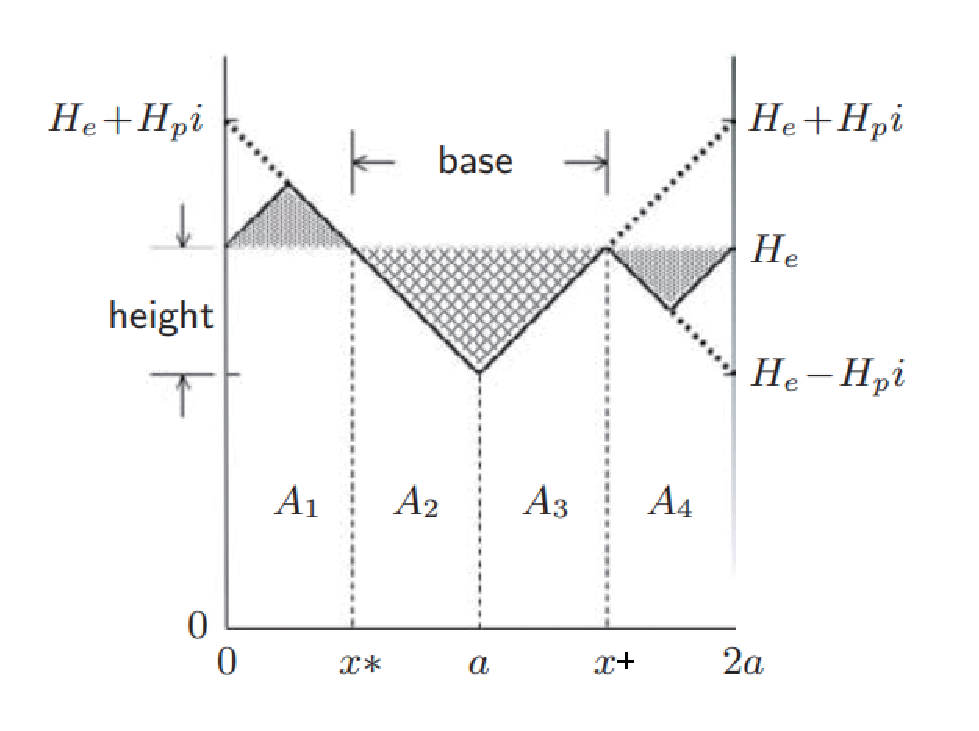
\includegraphics[scale=0.7]{chpt5/figs/fig5.14.eps}
	\caption{用以计算励磁的第五步之后的磁场特征。}
\end{figure}

\begin{figure}[htbp]
	\centering
	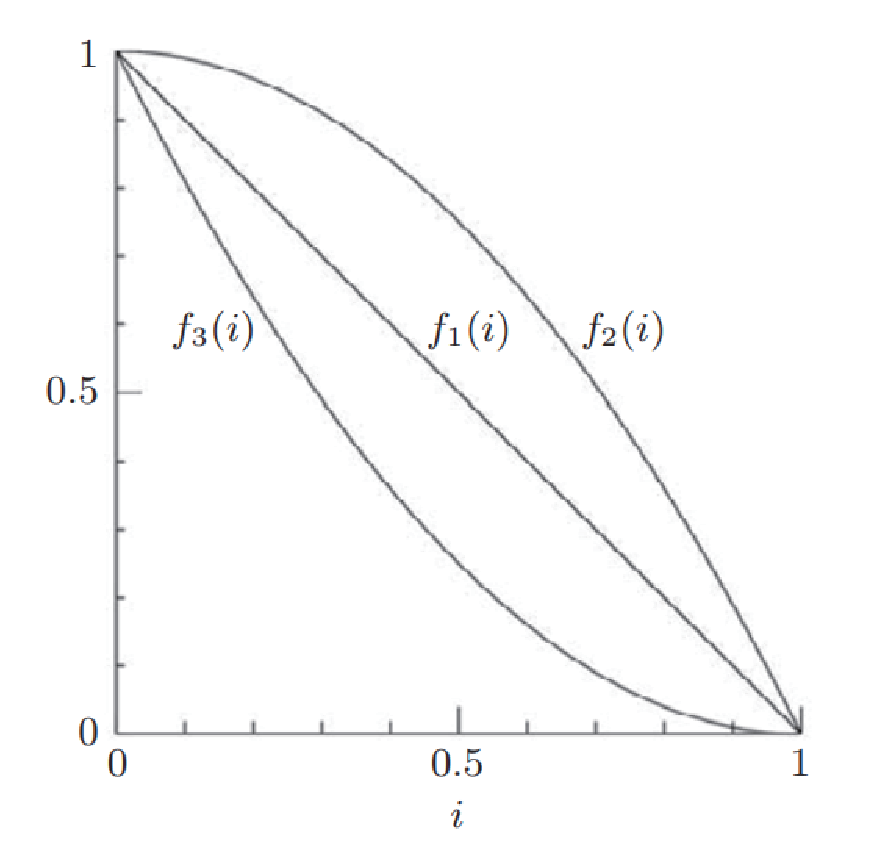
\includegraphics[scale=0.6]{chpt5/figs/fig5.15.eps}
	\caption{讨论5.1研究的三种归一化励磁 vs. 归一化电流关系。}
\end{figure}

\textbf{Magnetization Functions—Summary}

图5.15给出三个归一化磁化函数$f1(i), f2(i)$和$f3(i)$。其中,$i = I_t/I_c$。
很有意思的是,传输电流和外部磁场施加的不同顺序影响$M(i)$。
这些$f(i)$函数已得到试验验证[5.3, 5.4],故而Bean模型在提出之后很快就被人们接受了。


\subsection{讨论5.2:SQUID用于磁化测量}
SQUID (Superconducting Quantum Interference Device,超导量子干涉仪)是基于Josephson效应的一种电子
器件,可以极高的分辨率——单个磁通量子,幅值$2.0\times 10^{−15}\ \mathrm{Wb(Tm^2)}$——来测量磁场的变化。

一个典型的SQUID磁化测量装置的测试样品处于恒温,置于均匀磁场中。
测试样品在均匀场中前后移动;每一个周期内它切过分别位于测试样品两端的两个测试线圈。
每一个测试线圈中感应的电流产生的磁场由SQUID检测,反过来,这就是测试样品的磁化。
因为SQUID在低磁场环境下运行的最好( 不高于100 oersted或0.01 T),
通常要将之与测试样品的高场环境屏蔽。


\subsection{讨论5.3:“Bean细丝”中的磁化}
\subsubsection{第一部分:磁场平行于细丝轴}
我们使用Bean推导它的磁化表达式相同的假设,将一根直径$d_f$、无限长的超导细丝,
置于平行于细丝轴(z)d的外磁场$H_e\vec{i_z}$中。
对于置于$H_e\vec{i_z}$中的无限长细丝,应用Ampere定律:
\begin{equation}% page329 第1个
\frac{dH_{z}}{dr}\vec{\imath}_{\theta}=-J_{c}\vec{\imath}_{\theta}
\end{equation}
方程5.20表明,细丝内的轴向(z)磁场$H_s(r)$是r的线性函数,斜率为$J_c$。

\textbf{A. 初始态}

在$H_e \le H_p$时,where Hp is the critical-state field, the field within the filament,
Hs(r), is zero from r=0 to r∗=(df/2−He/Jc) and varies as Jcr from r∗ to df /2:
\begin{equation}% page329 第2个
H_{s}(r)=H_{e}\frac{r-r*}{\frac{d_{f}}{2}-r*}
\end{equation}
Note that r∗=0 when He=Hp, where Hp is the critical-state field:
\begin{equation}% page329 第3个
H_{p}=\frac{1}{2}J_{c}d_{f}
\end{equation}
Using steps similar to those taken with Eq. 5.4, we may compute the average
magnetic induction within the filament,$\~{B}_s$:
\begin{align}% page329 第4个
\tilde{B_{s}}&=\frac{4\mu_{o}}{\pi d_{f}^{2}}\int_{r*}^{\frac{d_{f}}{2}}H_{e}\frac{r-r*}{\frac{d_{f}}{2}-r*}(2\pi r)dr\\
&=\frac{8\mu_{o}H_{e}}{d_{f}^{2}(\frac{d_{f}}{2}-r*)}(\frac{1}{24}d_{f}^{3}-\frac{1}{8}d_{f}^{2}r*+\frac{1}{6}r*^{3})
\end{align}
Unlike in the case of a slab, where the integration may be performed geometrically
from Hs(x), here the “area” integration must be performed mathematically. By
inserting r∗=(df/2−He/Jc) into Eq. 5.23 and noting that Hp=Jcdf/2, we obtain:
\begin{equation}%page329 第5个
\frac{\tilde{B}_{s}}{\mu_{o}}=\frac{2H^{2}_{e}}{d_{f}J_{c}}-\frac{4H^{3}_{e}}{3(d_{f}J_{c})^{2}}=\\frac{H^{2}_{e}}{H_{P}}-\frac{H_{e}^{3}}{3H^{2}_{p}}
\end{equation}
根据定义$M=\~{B}_s/\mu_{0}-H_e$,我们有:
\begin{equation}%page329 第6个
-M=H_{e}-\frac{H^{2}_{e}}{H_{P}}+\frac{H^{3}_{e}}{3H^{2}_{p}}\quad(0\leq H_{e}\leq H_{P})
\end{equation}
Note that Eq. 5.25 is similar to, but clearly different from, Eq. 5.5 for the slab.

\textbf{B. 临界态及以上}

For He≥Hp the filament is in the critical state, and its magnetization is constant
and given from Eq. 5.25 with He=Hp:
\begin{equation}%page329 第7个
-M=\frac{1}{3}H_{p}=\frac{1}{3}(\frac{J_{c}d_{f}}{2})\quad(H_{e}\geq H_{p})
\end{equation}
The “magnetization factor” for the filament is 1/3; for the slab it is 1/2 (Eq. 5.6).

\subsubsection{第二部分:磁场垂直于细丝轴}
When the applied external field is perpendicular to the axis of a filament of diameter
df , the current distribution within the filament is complicated for He ≤Hp,
the critical field. For He≥Hp, a total current of Jcπd2
f/8 is induced flowing in the
+z-direction, and the same magnitude in the −z-direction. Figure 5.16 shows the
current distributions for: a) a Bean slab (2a); and b) a filament of diameter df .

We may compute the magnetization, M, by integrating the magnetic moment, mA,
per unit volume. Here, we derive expressions for the critical state magnetization
for a Bean slab of width 2a and a filament of diameter df .

\textbf{A. Bean板}

For a Bean slab in the critical state, the magnetic moment mA per unit length in
both z- and y-directions, from Jc(x) shown in Fig. 5.16a, is given by:
\begin{equation}%page330 第1个
m_{A}=\int_{0}^{a}2xJ_{c}(x)dx=J_{c}a^{2}
\end{equation}
The conductor volume per unit length in both z- and y-directions is 2a. Thus:
\begin{align*}%page330 第2个
M=\frac{m_{A}}{2a}=\frac{1}{2}J_{c}a\tag{5.27b}
\end{align*}
M given by Eq. 5.27b, except for the sign, is identical to that given by Eq. 5.6.

\textbf{B. 细丝}

For a filament of diameter df , the magnetic moment mA per unit length in the
z-direction, from Jc(x, y) shown in Fig. 5.16b, is given by:
\begin{equation}%page330 第3个
m_{A}=\int_{-\frac{d_{f}}{2}}^{\frac{d_{f}}{2}}2xJ_{c}(x,y)dxdy=\frac{1}{6}J_{c}d_{f}^{2}
\end{equation}
The conductor volume per unit length in the z-direction is πd2
f /4. Thus:
\begin{subequations}
	\begin{align*}
M&=\frac{\mathbf{4m_{A}}}{\pi d_{f}^{2}}=(\frac{4}{3\pi})J_{c}(\frac{d_{f}}{2})\simeq0.424J_{c}(\frac{d_{f}}{2})\sim0.5J_{c}a\\
H_{p}&=(\frac{8}{3\pi})J_{c}(\frac{d_{f}}{2})
	\end{align*}
\end{subequations}
This is nearly the same (8/3π∼1) as that for a Bean slab of thickness df .

\begin{figure}[htbp]
	\centering
	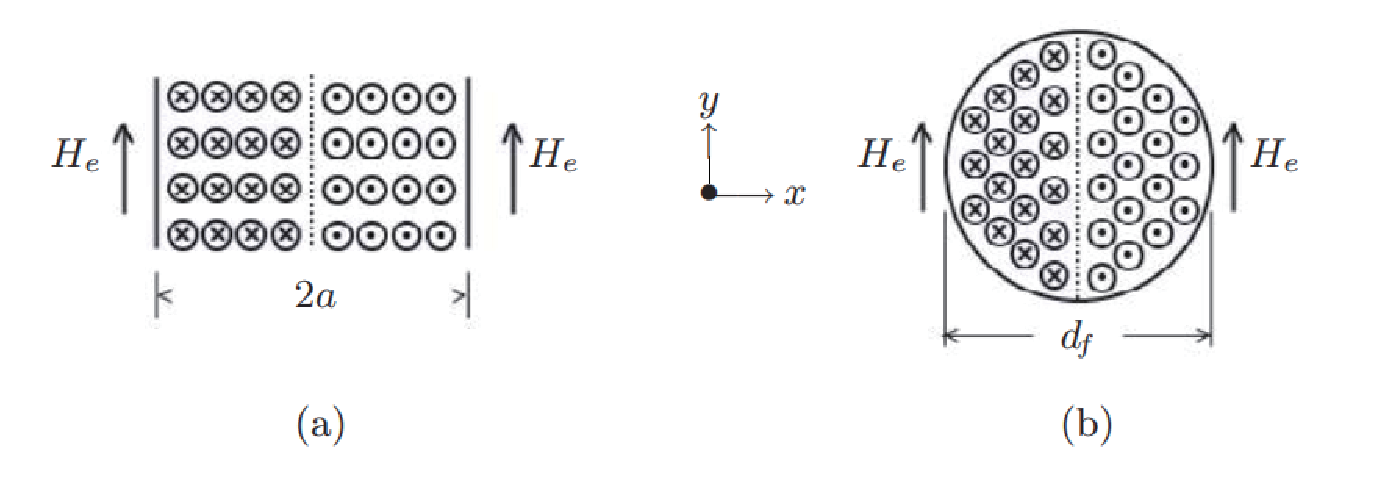
\includegraphics[scale=0.5]{chpt5/figs/fig5.16.eps}
	\caption{Induced current distributions in a) Bean slab of width 2a and b) an infinitely
		long filament of diameter dd, both subjected to an external field He in the y-direction.。}
\end{figure}

\subsection{讨论5.4:磁化中的$J_c$}
We demonstrate here how critical current density (Jc) data may be extracted
from magnetization (M) data. This method of extracting Jc data from M data
is quite useful when dealing with superconductor test samples too short for a
standard voltage vs. current measurement technique. Test samples too small for
V (I) measurement were common in the early days of HTS, and Bean’s model
discussed above was extremely useful.

In a V (I) measurement the sample must be “long” to: 1) generate a detectable
voltage with the very low electric field that defines the superconducting-to-normal
transition—the typical criterion is between 0.1 to $1\ \mathrm{\mu V/cm}$; and 2) keep the contact
resistance to the lead wires at each end of the test sample “low,” thereby preventing
excessive heating at the ends which might cause a premature normal transition.
The test samples should normally be at least 10mm long; perhaps under certain
circumstances they can be as short as 5 mm, but not much shorter than this. It
depends largely on the level of critical current.

Figure 5.8 presented the magnetization vs. applied field traces at 10 K, 20 K, and
30K of a short length (15mm) of copper/MgB2 composite wire of an equivalent
circular diameter of 1.038 mm[5.7]; the MgB2 itself has a diameter of 0.531 mm.
Here, the unit of magnetization is given in emu/cm3 corresponding to the total
wire diameter of 1.038 mm. The external field is along the wire axis, i.e., the same
configuration as in DISCUSSION 5.3 Part 1. To compute the superconductor’s Jc,
for example, at 10K in zero field, we treat the wire as a Bean rod of infinite length
and 0.531mm diameter. First, we convert emu/cm3 into the SI unit equivalent,
A/m, by multiplying it by 1000. (See Appendix I.)

At 10K in zero field, the magnetization, from Fig. 5.8, is 60 emu/cm3 or 60 kA/m.
To translate this to M corresponding to the volume of just the MgB2, we must
multiply 60 kA/m by (1.038/0.531)2 = 4.0. Solving Eq. 5.26 for Jc with M =
240 kA/m and df =5.31×10−4 m, we obtain:
\begin{align*}%page331 第5个
J_{c}(0\ \mathrm{T};10\ \mathrm{K})&=\frac{6\ \mathrm{M}(0\ \mathrm{T};10\ \mathrm{K})}{d_{f}}\\
&=\frac{6(240\times10^{3}\ \mathrm{A/m})}{(0.531\times10^{-3}\ \mathrm{m})}\\
&a=2.7\times10^{9}\ \mathrm{A/m^{2}}
\end{align*}


\subsection{问题5.1:磁化测量}
This problem applies the magnetization measurement technique discussed in 5.4 to
one of the four superconductors used in the Hybrid III SCM, to confirm that there
would be no flux jumping. The absence of flux jumping is one of the necessary
conditions for magnets that are not “cryostable”—this point will be discussed in
more detail in CHAPTER 6.

Table 5.1 presents specifications of the superconductor, a bare NbTi composite
strip with overall dimensions of 9.2mm width and 2.6mm thickness. (Not all
parameters in the table, e.g., twist pitch, are relevant for this problem.)

The test sample consisted of 52 (13×4) 100-mm long strips assembled in a rectangular
solid of square cross section, 38mm×38 mm, as shown in Fig. 5.17. Each
bare strip was electrically insulated with a thin tape. In the orientation shown
in Fig. 5.17a, each strip presents its narrow surface to the external magnetic induction
Be; in the orientation shown in Fig. 5.17b, each strip is broadside to
Be. The test sample assembly was placed inside a rectangular-bore (cross section
107mm×42mm) search coil set containing a primary search coil and two secondary
coils (Fig. 5.17c). The test assembly midplane coincided with that of the primary
search coil, whose midplane coincided with that of an external magnet generating
Be. The midplane-to-midplane distance between the primary and one of the
secondary coils was 70 mm. The primary coil had 500 turns of fine copper wire
over an axial distance of 40mm centered on its midplane; each secondary search
coil had 280 turns, extending an axial distance of 20mm centered on its midplane.
The turn density in the axial direction in each search coil was uniform.

When an external magnetic induction Be was swept at a rate of 0.05 T/s between
0 and 5T with the test sample at 4.2K with its orientation as in Fig. 5.17a, a
plot of −M (given in Vmz) vs. Be plot similar to that shown in Fig. 5.8 was
obtained. +Vmz is the integrator output proportional to −M, the negative of
the test sample magnetization. The effective integration time,$\tau_{it}$, was 1 s; the
balancing potentiometer’s constant k was 0.5. Assume negligible voltage drift.

\colorbox{red}{表5.1}


\begin{figure}[htbp]
	\centering
	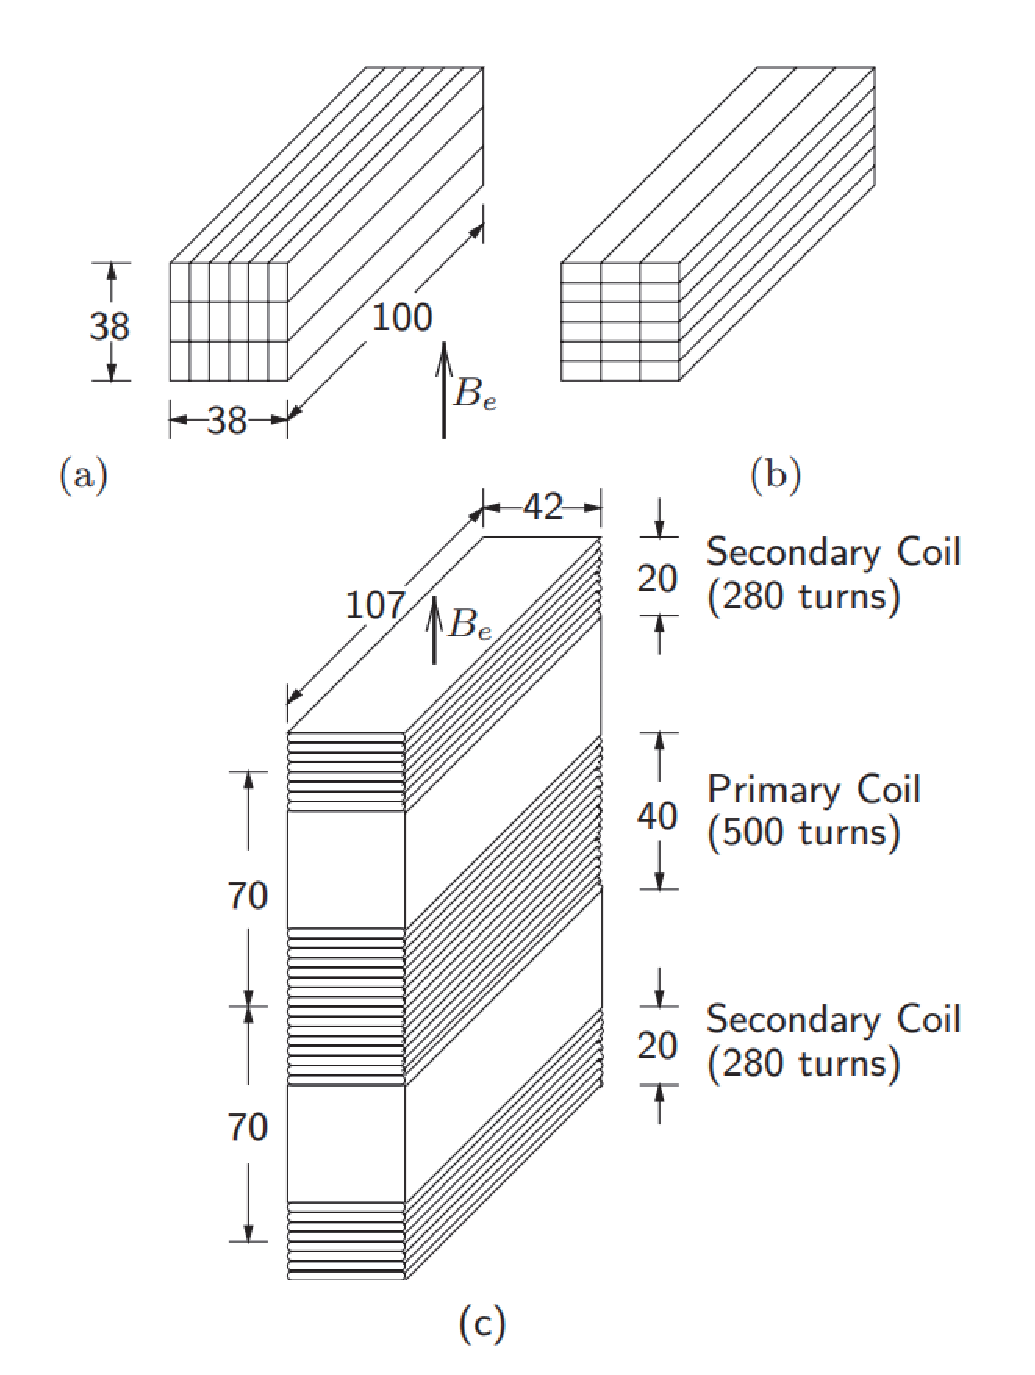
\includegraphics[scale=0.6]{chpt5/figs/fig5.17.eps}
	\caption{Magnetization measurement details, dimensions in mm.
		(a) Each strip presents its narrow surface to the external magnetic
		induction, Be; (b) Each strip is broadside to Be; (c) Search coil setup.。}
\end{figure}

a) Make a ballpark estimate of ΔVmz at Be∼2.5T (magnetization trace “width”
in Fig. 5.8, given in volts). Note that $\tau_{it}$ = 1 s and k = 0.5. Assume df = 2a,
where df is the filament diameter and 2a is the width of the Bean slab.

b) A 1.8-K measurement was performed by pumping on the cryostat and reducing
the liquid helium bath pressure to 12.6 torr. The technician who controlled
the cryostat pressure noticed that pressure control was more difficult,
because of an increased liquid boil-off rate, when the test sample orientation
was as in Fig. 5.17b rather than as in Fig. 5.17a. Is this an aberration or
does his observation make sense? Explain.

c) The z-component of the external induction Be over the radial space occupied
by the search coil may be approximated to vary as:
\begin{equation}%page333 第1个
B_{e}(z)\simeq B_{e}(0)[1-c(\frac{z}{z_{o}})^{2}]\qquad(5.30)
\end{equation}
where z◦ = 75 mm. Based on information you have, compute the value of c.

\subsubsection{问题5.1之解}
a) 方程5.13表明搜索线圈需要平衡;否则,正比于外施磁场的那一项会对视在磁化作贡献。既然图5.8中给出的$−M(H)$迹线并非上翘,可见搜索线圈已经获得平衡。

由方程5.14b有:
\begin{align*}%page334 第1个
V_{bg}(t)=(k-1)\mu_{o}N_{pc}A_{pc}\frac{dM}{dt}\tag{5.14b}
\end{align*}
由方程5.16c,我们有:
\begin{align*}%page334 第2个
\Delta V_{mz}=-f_{m}\frac{(k-1)\mu_{o}N_{pc}A_{pc}}{\tau_{it}}J_{c}a\tag{5.16c}
\end{align*}
我们有:$k$ = 0.5; $\tau_{it}$ = 1 s; $N_{pc}$ = 500; $A_{pc}$ = (13)(0.1 m)(2.6$\times 10^{−3}$ m) = 3.38$\times 10^{−3}\ \mathrm{m^2}$ 
[(0.1 m)$\times$(38$\times 10^{−3}$ m) = 3.8$\times 10^{−3}\ \mathrm{m^2}$也是可以接受的]; $f_m$ =(NbTi体积)/(总体积)= $1/(\gamma_{c/s} + 1)$ = 0.25。

\textbf{$J_c$的估计(4.2 K,2.5 T)}

从表5.1可知,在4.2 K和5 T时的$J_c$为$2.0\times 10^9\ \mathrm{A/m^2}$。
在给定温度下,基于方程1.3获得$J_c(B_e)$的近似值是业界普遍接受的:
\begin{align*}%page334 第3个
2.0\times10^{9}\ \mathrm{A/m^{2}}=\frac{J_{0}B_{0}}{5T+0.3T}\Rightarrow J_{0}B_{0}=10.6\times 10^{9}\ \mathrm{AT/m^{2}}
\end{align*}
式中,对NbTi,$B_0\sim$ 0.3 T。$J_0$是零场下的临界电流密度——通常是很难测量的。
于是,由5 T的$J_c$和$B_0$ = 0.3 T,我们首先可以得到$J_0 B_0$:
\begin{align*}%page334 第4个
2.0\times 10^{9}\ \mathrm{A/m^{2}}=\frac{J_{0}B_{0}}{5T+0.3T}\Rightarrow J_{0}B_{0}=10.6\times 10^{9}\ \mathrm{A/m^{2}}
\end{align*}
一旦获得了$J_0 B_0$,可以解出2.5 T时的$J_c$:
\begin{align*}%page334 第5个
J_{c}(2.5T)=\frac{10.6\times10^{9}\ \mathrm{AT/m^{2}}}{2.8T}=3.8\times 10^{9}\ \mathrm{A/m^{2}}
\end{align*}
向方程5.16c代入合适的值,有:
\begin{align*}%page334 第6个
\Delta V_{mz}&=-0.25\frac{(-0.5)(4\pi\times 10^{-7}\ \mathrm{H/m})(500)(3.38\times 10^{-3}\ \mathrm{m^{2}})}{1\ \mathrm{s}}\\
&\times(3.8\times 10^{9} A/m^{2})(50\times 1^{-6} m)\\
&\simeq 50\ \mathrm{mV}
\end{align*}

Because the strip is flattened from a round conductor by a process that squeezes
the conductor between rollers, the projected diameter of filaments in the direction
parallel to Be would be actually slightly less than the equivalent circular-area
radius, a = 50 $\mathrm{\mu m}$, which is used in the above computation for ΔVmz. If a radius
less than 50 $\mathrm{\mu m}$is used, ΔVmz would be less than 50 mV.

b) The anisotropic shape of the NbTi filaments makes magnetization in the orientation
of Fig. 5.17b greater than that in the orientation of Fig. 5.17a—the “effective”
a is greater. Thus there will be more magnetization loss.

If the aspect ratio of the filaments is the same as for the conductor, eddy current
loss will be proportional to$(a\.{H}_e)^2$in the orientation of Fig. 5.17b and$(b\.{H}_e)^2$
in the orientation Fig. 5.17a—review PROBLEM 2.8. Thus eddy current loss is
greater by a factor of (9.2/2.6)2 = 12.5 for Fig. 5.17b than for Fig. 5.17a.

The increased heat load on the helium due to higher magnetization and eddy
current losses causes a higher liquid helium boil-off rate; thus the technician’s
observation makes sense.

c) With balanced search coils, we have:
\begin{align*}%page335 第1个
N_{pc}A_{pc}(\frac{d\tilde{B}_{e}}{dt})_{pc}=N_{sc}A_{sc}(\frac{d\tilde{B}_{e}}{dt})_{sc}\tag{S1.2}
\end{align*}
%Because Apc = Asc, we have: Npc[˜Be]pc = Nsc[˜Be]sc. From symmetry, we consider
only the upper half (the unit mm is omitted in the following equations):
\begin{align*}%page335 第2个
[\tilde{B}_{e}]_{pc}=\frac{B_{e}(0)}{20}\int_{0}^{20}[1-c(\frac{z}{z_{0}})^{2}]dz\tag{S1.3a}
\end{align*}
\begin{align*}%page335 第3个
[\tilde{B}_{e}]_{sc}=\frac{B_{e}(0)}{20}\int_{60}^{80}[1-c(\frac{z}{z_{0}})^{2}]dz\tag{S1.3b}
\end{align*}
The Npc%[˜Be]pc = Nsc[˜Be]sc equality gives:
\begin{align*}%page335 第4个
\frac{250}{20}\int_{0}^{20}[1-c(\frac{z}{z_{0}})^{2}]dz&=\frac{280}{20}\int_{60}^{80}[1-c(\frac{z}{z_{0}^{2}})]dz\\\tag{S1.4}
250[20-\frac{c}{3}\frac{(20)^{3}}{(75)^{2}}]dz&=280[80-\frac{c}{3}\frac{(80)^{3}}{(75)^{2}}-60+\frac{c}{3}\frac{(60)^{3}}{(75)^{2}}]\\
5000-118.5c&=22400-8495.4c-16800+1584c\\
c&\simeq\frac{600}{4793}\simeq 0.125
\end{align*}


\subsection{讨论5.5:磁扩散和热扩散}
Before studying the flux jump criterion next in PROBLEM 5.2, we derive here basic
equations of magnetic and thermal diffusion to identify two diffusivities: magnetic
diffusivity, Dmg, and thermal diffusivity, Dth. The relative sizes of these two
diffusivities are quite different for electrically conductive normal metals ($D_{th}\gg D_{mg}$) and for Type II superconductors ($D_{th}\ll D_{mg}$). This condition of $D_{th}\ll D_{mg}$
in Type II superconductors makes the penetration of flux into a superconductor
an adiabatic process, leading, as we shall study in PROBLEM 5.2, to the criterion
for flux jumping.

To derive the magnetic diffusion equation, the applicable Maxwell’s equations are
Ampere’s law and Faraday’s law, both in differential forms:
\begin{align*}%page336 第1个
Ampere's\quad law:\quad \nabla\times\vec{H}=\vec{J}_{f}\tag{2.5}
\end{align*}
\begin{align*}%page336 第2个
Faraday's\quad law:\quad\nabla\times\vec{E}=-\frac{\partial\vec{B}}{\partial t}\tag{2.8}
\end{align*}
For the slab (width 2a) geometry, we can express Eqs. 2.5 and 2.8 as:
\begin{equation}%page336 第3个
Amperer's\quad law:\frac{\partial H_{y}}{\partial x}=J_{z}=\frac{E_{z}}{\rho_{e}}
\end{equation}
\begin{equation}%page336 第4个
Faraday's\quad law:\frac{\partial E_{z}}{\partial x}=\frac{\partial B_{y}}{\partial t}=\mu_{o}\frac{\partial H_{y}}{\partial t}
\end{equation}
where$\rho_e$is the material’s electrical resistivity. From Eqs. 5.31 and 5.32, we obtain:
\begin{align*}%page336 第5个
\rho_{e}\frac{\partial^{2}H_{y}}{\partial x^{2}}=\mu_{o}\frac{\partial H_{y}}{\partial t}
\end{align*}
\begin{equation}%page336 第6个
\frac{\rho_{e}}{\mu_{o}}\frac{\partial^{2}H_{y}}{\partial x^{2}}\equiv D_{mg}\frac{\partial^{2}H_{y}}{\partial x^{2}}=\frac{\partial H_{y}}{\partial t}
\end{equation}
Equation 5.33 is a magnetic diffusion equation, for which:
\begin{equation}%page336 第7个
D_{mg}=\frac{{\rho}_{e}}{\mu_{o}}
\end{equation}
Similarly, the one-dimensional thermal diffusion equation having constant thermal
properties is given by:
\begin{equation}%page336 第8个
k\frac{\partial^{2}T}{\partial x^{2}}=C\frac{\partial T}{\partial t}
\end{equation}
where k and C are, respectively, the material’s thermal conductivity and heat
capacity. Dividing both sides of Eq. 5.35a by C, we obtain:
\begin{align*}%page336 第9个
\frac{k}{C}\frac{\partial^{2}T}{\partial x^{2}}\equiv D_{th}\frac{\partial^{2}T}{\partial x^{2}}=\frac{\partial T}{\partial t}\tag{5.35b}
\end{align*}
Equation 5.35b is a thermal diffusion equation, for which:
\begin{equation}%page336 第10个
D_{th}=\frac{k}{C}\qquad(5.36)
\end{equation}
Note that Eq. 5.36 and 4.20 are equivalent, because$C=\rho c_p$

\colorbox{red}{表5.2}

Table 5.2 presents approximate values of electrical and thermal properties and
corresponding diffusivities at 4K and 80K for stainless steel and copper. From
Table 5.2 we can clearly see that stainless steel, a stand-in for normal-state superconductors,
and copper are opposite with respect to magnetic and thermal
diffusivities. Specifically, changes in magnetic field propagate quickly through
stainless steel, whereas temperature gradients are relatively slow to propagate;
hence, large nonuniform temperature distributions can be created in stainless steel
during changing magnetic fields. Physically, it means that magnetic heating happens
essentially adiabatically in Type II superconductors. In copper, the reverse
is true: the magnetic field diffuses very slowly, while any nonuniformity in temperature
is quickly “evened out.” Therefore, copper in intimate contact with Type
II superconductor can alleviate field-motion-induced instability in Type II superconductors.
This thinking is the essence of dynamic stability, one of the stability
criteria developed during the 1960s and 1970s [5.8] and applied also to HTS in the
late 1980s [5.9].

\subsection{问题5.2:磁通跳跃判据}
This problem deals with the derivation of the critical conductor size above which
flux jumping will occur. Flux jumping was once a major source of instabilities in
the first superconducting magnets of engineering significance in the early 1960s
[5.10]. Flux jumping is a thermal instability peculiar to a Type II superconductor
that permits the magnetic field to penetrate its interior. A time-varying magnetic
field,$\.{H}_e$, at the conductor surface induces an electric field$\vec{E}$in the conductor,
which interacts with the supercurrent (density Jc). This$\vec{E}\cdot \vec{J}_c$interaction heats
the conductor. Since Jc decreases with temperature, the field (flux) penetrates
further into the conductor, generating more heat, which further decreases Jc. The
field penetration and temperature rise can cascade until the conductor loses its
superconductivity. This thermal runaway event is called a flux jump.

a) Using the Bean model and computing the $\vec{E}\cdot \vec{J}_c$ interaction over the positive
half (0 ≤ x ≤ a) of the slab, show that an expression for the dissipative energy
density,$e_\phi$[J/m3], generated within the slab when the critical current density
Jc is suddenly decreased by |ΔJc| is given by:
\begin{equation}%page338 第1个
e_{\phi}=\frac{\mu_{o}J_{c}|\Delta J_{c}|a^{2}}{3}
\end{equation}
Note that the entire slab is in the critical state with its surface (±a) exposed
to an external field of$H_e\vec{i}_y$.

b) Derive Eq. 5.37 by computing the Poynting energy flow into the slab at x = a
and equating it with the change in magnetic energy storage and dissipation
energy$E_\phi$in the positive half of the slab.

c) To relate ΔJc to an equivalent temperature rise in the conductor, we may
assume a linear temperature dependence for Jc(T):
\begin{equation}%page338 第2个
J_{c}(T)=J_{c_{o}}(\frac{T_{c}-T}{T_{c}-T_{op}})
\end{equation}
where Jc◦ is the critical current density at the operating temperature Top. Tc
is the critical temperature at a given magnetic induction B◦. From Eq. 5.38,
ΔJc in Eq. 5.37 may be related to an equivalent temperature rise ΔT:
\begin{equation}%page338 第3个
\Delta J_{c}=-J_{c_{o}}(\frac{\Delta T}{T_{c}-T_{op}}
\end{equation}
Now, by requiring that $\Delta T_s=e_\phi/\~{C}_s\le \Delta T$, where$\~{C}_s$is the superconductor’s
average heat capacity [J/m3 K] in the range from Top to Tc, show thermal
stability implies a critical slab half width ac of:
\begin{equation}%page338 第4个
a_{c}=\sqrt{\frac{3\tilde{C}_{s}(T_{c}-T_{op})}{\mu_{o}J_{c_{o}}^{2}}}
\end{equation}


\subsubsection{问题5.2之解}
a) Because of symmetry about x = 0, we
shall consider only one half of the slab, between
x = 0 and x = a. As illustrated in Fig. 5.18,
the solid line corresponds to Hs1(x), which
gives the initial field distribution within the
slab, with J =Jc. The dotted line corresponds
to Hs2(x) for the slab carrying Jc−|ΔJc|. Note
that the field at the surface is He in both cases.
We thus have:

\begin{figure}[htbp]
	\centering
	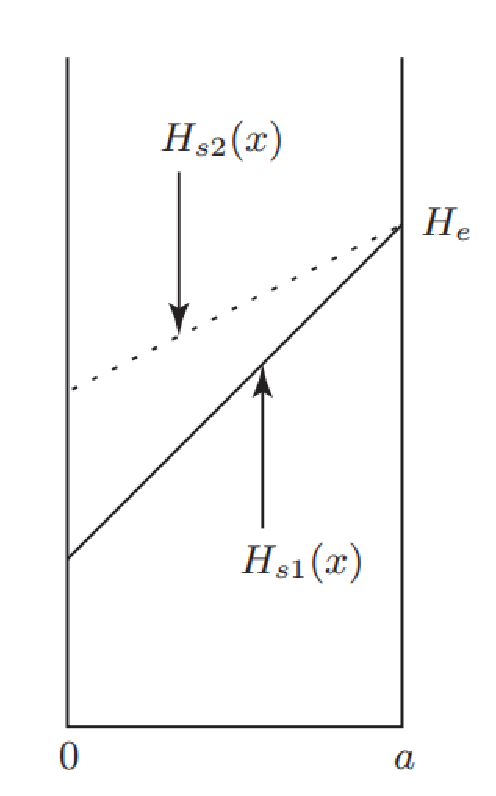
\includegraphics[scale=0.5]{chpt5/figs/fig5.18.eps}
	\caption{磁场特征。}
\end{figure}

\begin{align*}%page339 第1个
H_{s1}(x)=H_{e}+J_{c}(x-a)\tag{S2.1a}
\end{align*}
\begin{align*}%page339 第2个
H_{s2}(x)=H_{e}+(J_{c}-| \Delta J_{c}|)(x-a)\tag{S2.1b}
\end{align*}
Because there is a change in magnetic field
within the slab, an electric field$\vec{E}$is generated,
which from Faraday’s law of induction is
given by:
\begin{align*}%page339 第3个
\oint_{C}\vec{E}\cdot d\vec{s}=-\mu_{o}\int_{S}\frac{\triangle H_{s}(x)\vec{\imath}_{y}\cdot d\vec{A}}{\Delta t} \tag{S2.2}
\end{align*}
From symmetry we have$\vec{E}(x = 0) = 0$ and$\vec{E}$points in the z-direction. ΔHs(x)
is given by:
\begin{align*}%page339 第4个
\Delta H_{s}(x)&=H_{s2}(x)-H_{s1}(x)\\
&=|\Delta J_{c}|(a-x)\tag{S2.3}
\end{align*}
联立方程S2.2和S2.3,有:
\begin{align*}%page339 第5个
E_{z}(x)&=\mu_{o}\frac{|\Delta J_{c}|}{\Delta t}\int_{0}^{x}(a-x)dx\\
&=\mu_{o}\frac{|\Delta J_{c}|}{\Delta t}(ax-\frac{x^{2}}{2})\tag{S2.4}
\end{align*}
Dissipation power density, p(x), is given by Ez(x)Jc; the total energy density per
unit length dissipated in the slab or per unit slab surface area in the y-z plane,$E_\phi$
[J/m2], is given by:
\begin{align*}%page339 第6个
\varepsilon_{\phi}&=\int_{0}^{a}p(x)\Delta tdx\\
&=\mu_{o}J_{c}|\Delta J_{c}|\int_{0}^{a}(ax-\frac{x^{2}}{2})dx=\frac{\mu_{o}J_{c}|\Delta J_{c}|a^{3}}{3}\tag{S2.5}
\end{align*}
The average dissipation energy density,$e_\phi$ is given by$E_\phi/a$:
\begin{align*}%page339 第7个
e_{\phi}=\frac{\mu_{o}J_{c}|\Delta J_{c}|a^{2}}{3}\tag{5.37}
\end{align*}

b) The Poynting energy flux [J/m2] in the y-z plane into the slab (in the −xdirection)
at x = a is equal to the change in magnetic energy storage flux ΔEm
[J/m2] and dissipation energy flux$E_\phi$ in the slab. Thus:
\begin{align*}%page340 第1个
\int S_{x}(a)dt=\Delta E_{m}+\varepsilon_{\phi}\tag{S2.6}
\end{align*}
通过在$x=a$处计算$\vec{S}=\vec{E}\times\vec{H}$可以确定$\vec{S}$的方向。在$x=a$处,
$\vec{H}=H_e \vec{i_y}$;由方程S2.4得到的$E_z(x)$,可得:
\begin{align*}%page340 第2个
E_{z}(a)=\mu_{o}\frac{|\Delta J_{c}|a^{2}}{2\Delta t}\tag{S2.7}
\end{align*}
于是:
\begin{align*}%page340 第3个
\vec{S}(a)=\mu_{o}\frac{|\Delta J_{c}|a^{2}}{2\Delta t}\vec{\imath}_{z}\times H_{e}\vec{\imath}_{y}=-\mu_{o}\frac{H_{e}|\Delta J_{c}|a^{2}}{2\Delta t}\tag{S2.8}
\end{align*}
As expected,$\vec{S}(a)$points in the −x-direction; energy indeed flows into the slab.
Thus:
\begin{align*}%page340 第4个
\int S_{x}(a)dt=\mu_{o}\frac{H_{e}|\Delta J_{c}|a^{2}}{2}\tag{S2.9}
\end{align*}
The difference in magnetic energy flux ΔEm in the slab is given by:
\begin{align*}%page340 第5个
\Delta E_{m}&=\frac{\mu_{o}}{2}\int_{0}^{a}[H_{s2}^{a}(x)-H_{s1}^{2}(x)]dx\\\tag(S2.10)
&=\frac{\mu_{o}}{2}\int_{0}^{a}\{[H_{e}+(J_{c}-|\Delta J_{c}|)(x-a)]^{2}-[H_{e}+J_{c}(x-a)]^{2}\}dx\\
&=\frac{\mu_{o}}{2}\int_{0}^{a}[-2H_{e}|\Delta J_{c}|(x-a)-2J_{C}|\Delta J_{c}|(x-a)^{2}+|\Delta J_{c}|^{2}(x-a)^{2}]dx
\end{align*}
Neglecting the |ΔJc|2 term in the above integral, we obtain:
\begin{align*}%page340 第6个
\Delta E_{m}=\mu_{o}(\frac{H_{e}|\Delta J_{c}|a^{2}}{2}-\frac{J_{c}|\Delta J_{c}|a^{3}}{3})\tag{S2.11}
\end{align*}
From Eq. S2.6, we have:
\begin{align*}%page340 第7个
\varepsilon_{\phi}=\int S_{x}(a)dt-\Delta E_{m}\tag{S2.12}
\end{align*}
Combining Eqs. S2.9, S2.11, and S2.12, we obtain:
\begin{align*}%page340 第8个
\varepsilon_{\phi}&=\mu_{o}\frac{H_{e}|\Delta J_{c}|a^{2}}{2}-\mu_{o}(\frac{H_{e}|\Delta J_{c}|a^{2}}{2}-\frac{J_{c}|\Delta J_{c}|a^{3}}{3})\\
&=\mu_{O}\frac{J_{c}|\Delta J_{c}|a^{3}}{3}\tag{S2.13}
\end{align*}
Equation S2.13 leads directly to Eq. 5.37:
\begin{align*}%page340 第9个
e_{\phi}=\frac{\varepsilon_{\phi}}{a}=\frac{\mu_{o}J_{c}|\Delta J_{c}|a^{2}}{3}\tag{5.37}
\end{align*}

c) As given by Eq. 5.38, Jc(T) is a decreasing function of temperature. We thus
have:
\begin{align*}%page341 第1个
\Delta J_{c}=-J_{c_{c}}(\frac{\Delta T}{T_{c}-T_{op}})\tag{5.39}
\end{align*}
From Eq. 5.39, we have:
\begin{align*}%page341 第2个
|\Delta J_{c}|=\frac{J_{c_{o}}\Delta T}{T_{c}-T_{op}}\tag{S2.14}
\end{align*}
Replacing Jc with Jc◦ in Eq. 5.37 and combining it with Eq. S2.14, we obtain:
\begin{align*}%page341 第3个
e_{\phi}=\frac{\mu_{o}J_{c_{o}}^{2}\Delta T a^{2}}{3(T_{c}-T_{op})}\tag{S2.15}
\end{align*}
Note that$e_{\phi}$is proportional not only to ΔT but also, more importantly, to a2.
Under adiabatic conditions, the dissipation energy density$e_{\phi}$increases the superconductor’s
temperature by ΔTs, given by:
\begin{align*}%page341 第4个
\Delta T_{s}=\frac{e_{\phi}}{\tilde{C}_{s}}>0\tag{S2.16}
\end{align*}
$\tilde{C}_{s}$is the superconductor’s average heat capacity [J/m3 K] in the temperature
range from Top to Tc. Combining Eqs. S2.15 and S2.16, and requiring ΔTs < ΔT
for thermal stability, we have:
\begin{align*}%page341 第5个
\frac{\Delta T_{s}}{\Delta T}<\frac{\mu_{o}J_{c_{o}}^{2}a^{2}}{3\tilde{C}_{s}(T_{c}-T_{op})}\tag{S2.17}
\end{align*}
For a given superconducting material and operating temperature, a is the only
parameter that can be varied by the magnet designer to satisfy Eq. S2.17. That
is, thermal stability can be satisfied only if the slab half-width a is less than the
critical size ac, given by:
\begin{align*}%page341 第6个
a_{C}=\sqrt{\frac{3\tilde{C}_{s}(T_{c}-T_{op})}{\mu_{o}J_{c_{o}}^{2}}}\tag{5.40}
\end{align*}
Equation 5.40 is applied to compute approximate values of ac for NbTi (LTS) operating
at 4.2K and YBCO (HTS) operating at 77.3 K. Table 5.3 lists approximate
values of parameters appearing in Eq. 5.40 for both superconductors.

We may conclude that for a circular filament of NbTi, ac=140 $\mu m$means a critical
diameter of ∼300 $\mu m$(Eq. 5.29) and a coated YBCO tape of width 8 mm.


\colorbox{red}{表5.3}

\subsection{问题5.3:磁通跳跃}
The magnetization vs. ambient field trace shown in Fig. 5.19 was obtained with a
monofilament Nb-Zr wire (0.5mm$\phi$) at 4.2K carrying no transport current. (In
the early 1960s, superconductors based on alloys of niobium and zirconium, Nb-Zr,
preceeded Nb-Ti. Shortly after a composite superconductor became the standard
form for magnet-grade superconductors in the mid 1960s, Nb-Ti (now more commonly
designated NbTi), being much easier to co-process with copper than Nb-Zr,
replaced Nb-Zr.) Note that both ordinate (magnetization) and abscissa (field) are
given in non-SI units. Use Bean’s model and treat the wire, of diameter df, as a
slab of thickness 2a.

a) Show that the field interval, ΔHf , indicated in the trace, is consistent with
the measured magnitude of magnetization.

b) Estimate the dissipation energy density,$e_{\phi}$[J/m3], resulting from the flux
jump labeled A in Fig. 5.19. First, show that$e_{\phi}$is given by:
\begin{equation}%page342 第1个
e_{\phi}=\frac{(\mu_{o}J_{p})^{2}}{6\mu_{o}}
\end{equation}

c) Estimate the temperature rise for flux jump A. Assume the heat capacity of
Nb-Zr to be independent of temperature and equal to 6 kJ/m3 K.

\begin{figure}[htbp]
	\centering
	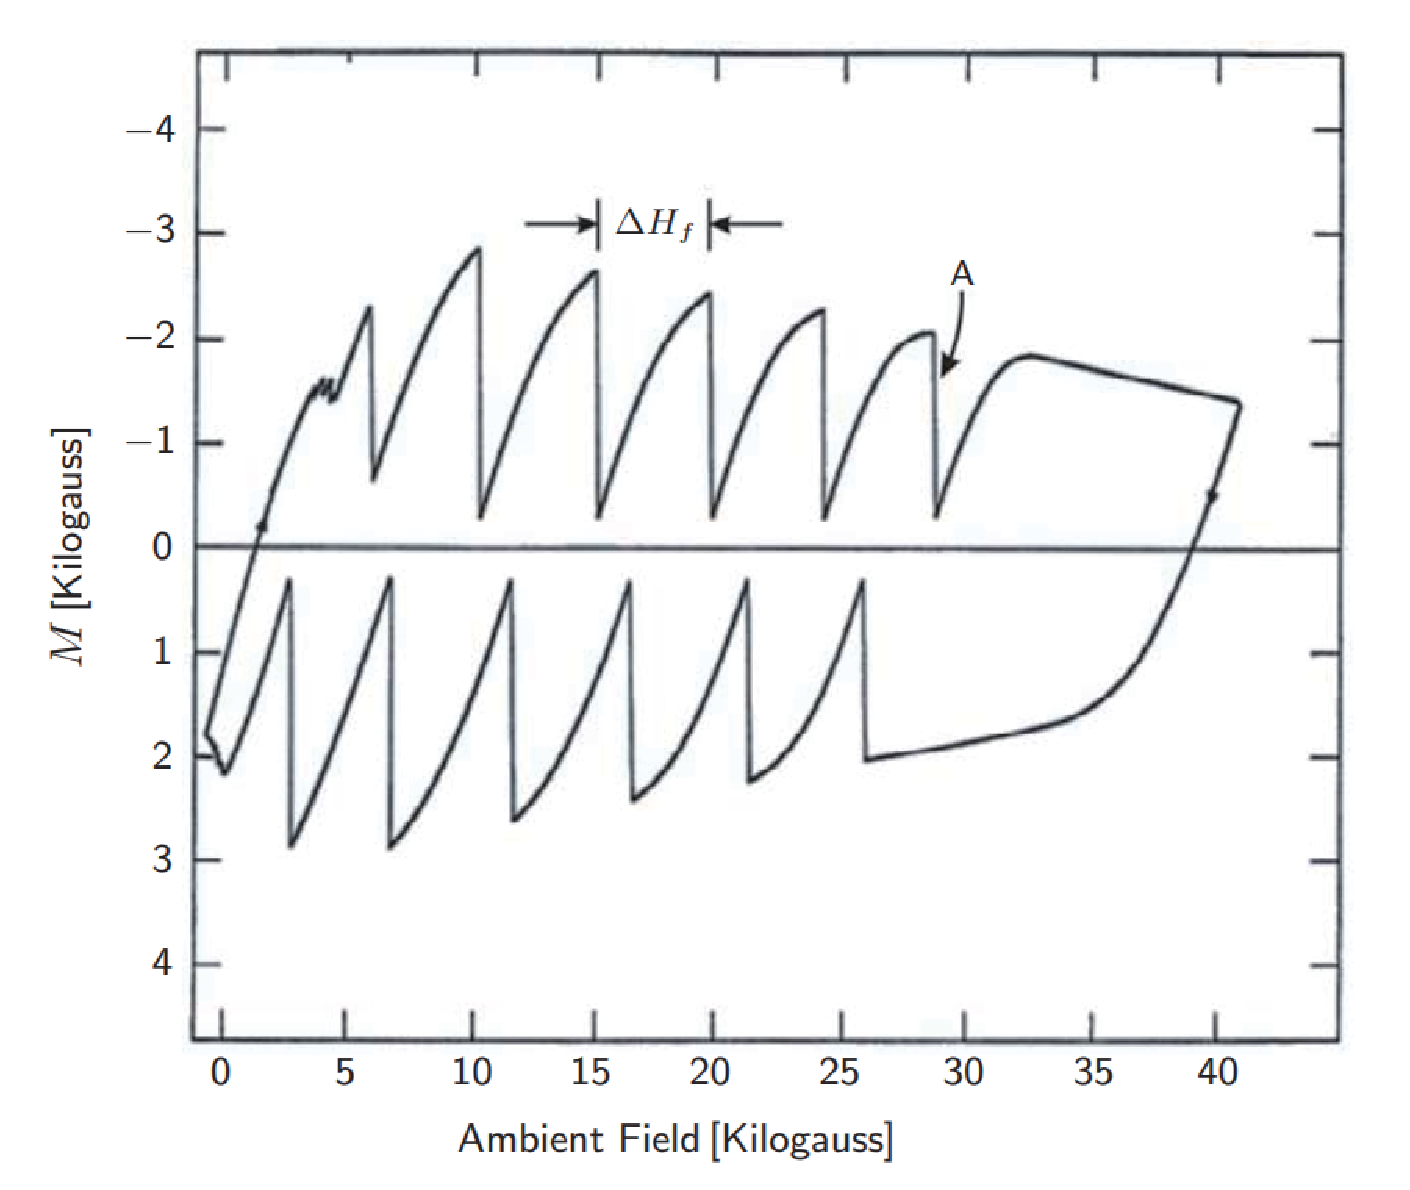
\includegraphics[scale=0.5]{chpt5/figs/fig5.19.eps}
	\caption{Magnetization vs. ambient field trace for a 0.5-mm dia. Nb-Zr monofilament。}
\end{figure}


\subsubsection{问题5.3之解}
a) From Bean’s model, flux jumping can occur every Hp. Clearly, Hp = ΔHf ,
where ΔHf is indicated in Fig. 5.19. Also, full magnetization for a slab is Hp/2.

从图5.19可知,$\Delta H_f\simeq$ 5k gauss,$\mu_{0}\Delta H_f$=0.5 T。图中还给出,
$H_p/2\simeq$ 2.5k gauss,是$\Delta H_f$的一半。他们是一致的。

b) We can derive the flux jump energy density,$e_{\phi}$, using the Poynting energy
balance:$e_s=e_{\phi}+\Delta e_m$, where es is the Poynting energy density entering the
superconductor at x=a, and$\Delta e_m$is its change in stored magnetic energy density.
Let’s consider only 0 ≤ x ≤ a. ΔH(x) within the slab is given by:
\begin{align*}%page343 第1个
\Delta H(x)=H_{p}\frac{(a-x)}{a}\tag{S3.1}
\end{align*}
由S3.1,可得:
\begin{align*}%page343 第2个
E(x)=\mu_{o}\frac{H_{p}}{\Delta t}\int_{0}^{x}\frac{a-x}{a}dx=\frac{\mu_{o}H_{p}}{a\Delta t}(ax-\frac{x^{2}}{2})\tag{S3.2}
\end{align*}
这样,在$x=a$处$\vec{S}$为:
\begin{align*}%page343 第3个
\vec{S}(a)=-\frac{\mu_{o}}{2\Delta t}H_{p}aH_{e}\vec{\imath}_{x}\tag{S3.3}
\end{align*}
$\vec{S}(a)$is directed towards the slab, and the Poynting energy density es is given by:
\begin{align*}%page343 第4个
e_{s}=\frac{\int S_{x}(a)dt}{a}=\frac{\mu_{o}}{2}H_{p}H_{e}\qquad(S3.4)
\end{align*}
The stored magnetic energy density after flux jumping (em2) is μ◦H2
e /2. The stored magnetic energy density before flux jumping, em1, is given by:
\begin{align*}%page343 第5个
e_{m1}=\frac{\mu_{o}}{2a}\int_{0}^{a}[H_{e}+J_{c}(x-a)]^{2}dx\tag{S3.5}
\end{align*}
\begin{align*}%page343 第6个
=\frac{\mu_{o}}{2a}(H_{e}^{2}a-H_{e}J_{c}a^{2}+\frac{J_{c}^{2}a^{3}}{3})=\frac{\mu_{o}}{2}H_{e}^{2}-\frac{\mu_{o}}{2}H_{e}H_{p}+\frac{\mu_{o}}{6}H_{p}^{2}\tag{S3.6}
\end{align*}
\begin{align*}%page343 第7个
\Delta e_{m}=e_{m2}-e_{m1}=\frac{\mu_{o}}{2}H_{e}H_{p}-\frac{\mu_{o}}{6}H_{p}^{2}\tag{S3.7}
\end{align*}
因为$e_\phi=e_s-\Delta e_m$,我们有:
\begin{align*}%page343 第8个
e_{\phi}=\frac{\mu_{o}}{2}H_{p}H_{e}-\frac{\mu_{o}}{2}H_{e}H_{p}+\frac{\mu_{o}}{6}H_{p}^{2}=\frac{\mu_{o}}{6}H_{p}^{2}\tag{S3.8}
\end{align*}
Equation S3.8 may be expressed as:
\begin{align*}%page343 第9个
e_{\phi}=\frac{(\mu_{o}H_{p})^{2}}{6\mu_{o}}\tag{5.41}
\end{align*}
Inserting μ◦Hp=0.5T into Eq. 5.41:
\begin{align*}%page343 第10个
e_{\phi}\simeq\frac{(0.5T)^{2}}{(6)(4\pi\times10^{-7}\ \mathrm{H/m})}\simeq33\times10^{3}\ \mathrm{J/m^{3}}
\end{align*}

c) $e_\phi = C_s \Delta T_s;33\times 10^3= 6\times 10^3 \Delta T_s$。我们解得:
$\Delta T_s$=5.5 K。这足以令超导体进入正常态了。


\subsection{问题5.4:导线换位}
如问题5.2中所讨论的,为了避免磁通跳跃,要求导体直径要小于$2a_c$,对NbTi,该值为$\sim 250\ \mathrm{\mu m}$。NbTi线的典型$J_{c_o}$是$2\times 10^9\ \mathrm{A/m^2}$(4.2 K和5 T),
$250\ \mathrm{\mu m}$直径的线的临界电流仅为$\sim 100$ A——如果使用单线,对大多数磁体应用都是不够的。
1960s末提出了使用多根线制造导体的思想:每一根线足够细以避免产生磁通跳跃,而后附着与常规金属上。
这种方法当时就造出来高达1000 A临界电流的线。现在已经可以造出50 kA的导体了。

In early (c. 1969) “multifilamentary” conductors, wires were untwisted. Coupling
between filaments caused the wire as a whole to flux jump, despite each filament
being small enough to satisfy the size criterion (Eq. 5.40). PROBLEM 5.5 deals
with such conductors. Results of a study of multifilamentary conductors, analytical
and experimental, by Wilson and others at the Rutherford Laboratory in the late
1960s launched a new era of multifilamentary conductors [5.11].

Simply stated, when filaments are embedded in a conductive metal (e.g., copper)
and subjected to a time-varying magnetic field, the filaments are electrically coupled
according to Faraday’s law. They then act as a single entity with an effective
conductor diameter nearly as great as that of the entire conductor. The basic
premise of the flux jumping criterion for isolated filaments is thus violated in an
untwisted multifilamentary conductor. In order to eliminate flux jumping in multifilamentary
conductors, filaments must be decoupled. Twisting of the wires, or
more ideally transposition of the filaments (or strands of a multi-strand conductor),
can do the trick of filament decoupling.

Consider a two-dimensional conductor model comprised of two Bean slabs, each
df wide, separated by a copper slab of width 2w and electrical resistivity ρcu.
Figure 5.20 shows the conductor as seen looking down the z-axis. Note that unlike
the one-dimensional Bean slab which extends into infinity in both the y- and zdirections,
this conductor is$2\ell$long in the y-direction.

\begin{figure}
	\centering
	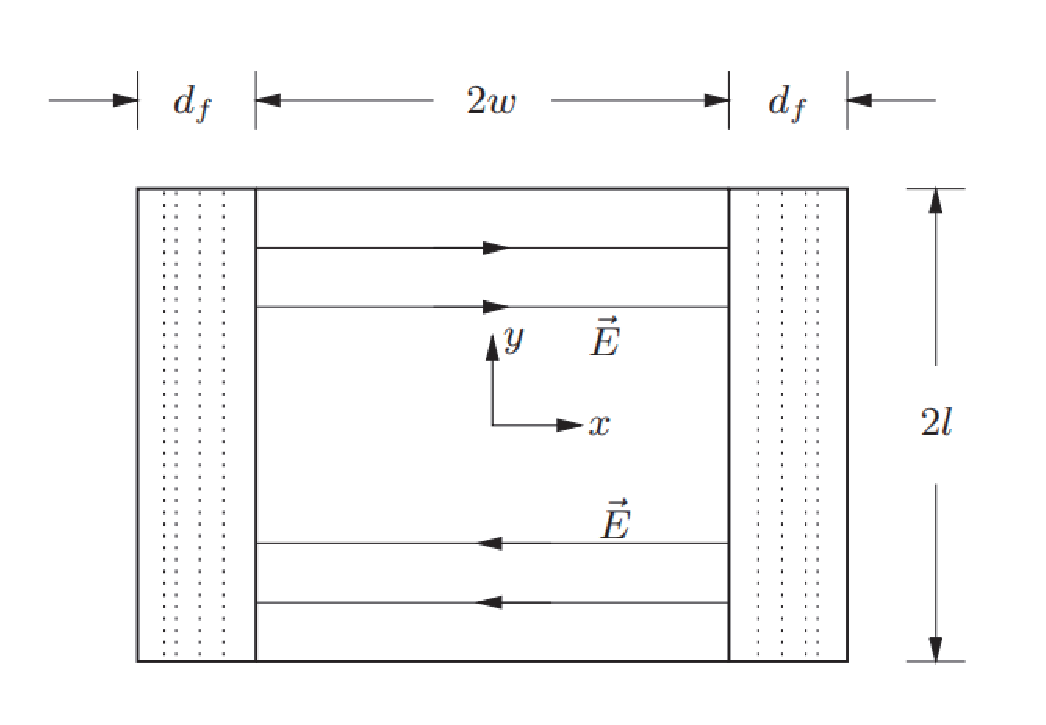
\includegraphics[scale=0.6]{chpt5/figs/fig5.20.eps}
	\caption{Two-dimensional conductor consisting of a normal
		metal slab sandwiched between two Bean slabs.}
\end{figure}

Suppose the conductor is subjected to a spatially uniform, time-varying magnetic
field pointed in the z-direction,$\.{H}_{0z}\vec{i_z}$

a) Show that the x-directed electric field within the copper slab, E1x, varies
with y as given by:
\begin{equation}%page345 第1个
E_{1x}=\mu_{o}\dot{H}_{0z}y\qquad(5.42)
\end{equation}
Assume the electric field in each superconducting slab to be zero—strictly
speaking it is not, but compared with that in the copper, it is extremely
small; hence the approximation of zero$\vec{E}$field is valid. Also assume the field
to be quasi-static. Under these assumptions, it is apparent that the$\vec{E}$field
in the copper, as indicated in Eq. 5.42, has only an x component.

b) Show that the net current flowing through the copper (per unit conductor
depth in the z-direction), Icp [A/m], from one superconducting slab to the
other superconducting slab, over one half conductor length (from y = 0 to$y=\ell$), is given by:
\begin{equation}%page345 第2个
I_{cp}=\int_{0}^{\ell}J_{cu}dy=\frac{\mu_{o}\dot{H}_{0z}}{\rho_{cu}}\int_{0}^{\ell}ydy=\frac{\mu_{o}\dot{H}_{0z}\ell^{2}}{2\rho_{cu}}\quad(5.43)
\end{equation}

c) At a critical length$\ell_c$, the net current Icp given by Eq. 5.43, becomes equal
to Jcdf , the slab’s critical current (per unit conductor depth). Show that
the critical length$\ell_c$is:
\begin{equation}%page345 第3个
\ell_{c}=\sqrt{\frac{2\rho_{cu}J_{c}d_{f}}{\mu_{o}\dot{H}_{0z}}}\qquad(5.44)
\end{equation}

d) Multifilamentary superconductors for 60-Hz power applications must have a
filament size (df ) that is extremely small, in the range 0.1∼0.5 μm, which
is even smaller than the wavelength of visible light (∼0.7$\mu m$). This extremely
small size is required to keep “manageable” the hysteresis energy,
generated within each filament every time a magnetic field is cycled. (As
will be discussed in CHAPTER 6, hysteresis loss per cycle of field excitation
is proportional to filament diameter.)

Compute$\ell_c$for a typical “submicron” superconductor having the following
parameters:
% ρm = 30nΩm; Jc = 2GA/m2; df = 0.2 μm; μ◦ ˙H0z = 2 kT/s
(equivalent to a sinusoidal excitation of 5-T amplitude magnetic induction
at 60 Hz).$\rho_m$is the electric resistivity of the matrix, which is generally a
copper-nickel alloy.

e) Compute the number of filaments required for a submicron multifilamentary
conductor with a filament diameter of 0.2$\mu m$ having a critical current of
100 A. Use the same values of parameters given in d).

\subsubsection{问题5.4之解}
a) From Faraday’s law, applied under the quasi-static assumption, we have:
\begin{align*}%page346 第1个
\frac{\partial E_{1y}}{\partial x}-\frac{\partial E_{1x}}{\partial y}=-\mu_{o}\dot{H}_{0z}\tag{S4.1}
\end{align*}
Because$\vec{E}$is zero in the superconducting slabs, Ey = 0 at x = ±w, forcing E1y = 0
everywhere in the copper slab. Thus:
\begin{align*}%page346 第2个
E_{1x}=\mu_{o}\dot{H}_{0z}y\tag{5.42}
\end{align*}

b) Once the E field is known, the current density Jcu in the copper slab is given
by: Jcu = E1x/ρcu. The net current flowing in the copper from one superconducting
slab to the other over half the conductor length is given by:
\begin{align*}%page346 第3个
I_{cp}=\int_{0}^{\ell}J_{cu}dy=\frac{\mu_{o}\dot{H}_{0z}}{\rho_{cu}}\int_{0}^{\ell}ydy=\frac{\mu_{o}\dot{H}_{0z}\ell^{2}}{2\rho_{cu}}\tag{5.43}
\end{align*}

c) Equating Icp given by Eq. 5.43 with Jcdf and solving for$\ell_c$, we have:
\begin{align*}%page346 第4个
\ell_{c}=\sqrt{\frac{2\rho_{cu}J_{c}d_{f}}{\mu_{o}\dot{H}_{0z}}}\tag{5.44}
\end{align*}

d) Inserting appropriate values into Eq. 5.44, we obtain:
\begin{align*}%page346 第4个
\ell_{c}=110\ \mathrm{\mu m}
\end{align*}
In typical submicron strands, the twist pitch length is thus ∼100$\mu m$. This means
that the diameter of such strands, by mechanical requirements, should be ∼1$\mu m$;
actually a thermal-magnetic stability criterion, similar to the flux jump criterion,
requires it to be even smaller than 1$\mu m$. This is because the strands, to reduce
coupling losses, use Cu-Ni alloys as the matrix materials, resulting in a magnetic
diffusion time constant that is smaller than the thermal diffusion time constant.

e) Critical current (Ic), critical current density (Jc), filament number (Nf ) and
diameter (df ) in a multifilamentary conductor are related by:
\begin{align*}%page346 第4个
I_c=N_f\frac{\pi d_f^2}{4} J_c \tag{S4.2}
\end{align*}
Solving for Nf from Eq. S4.2 with appropriate values of parameters, we obtain:
\begin{align*}%page346 第5个
N_{f}&=\frac{4I_{c}}{\pi d_{f}^{2}J_{c}}=\frac{4(100A)}{\pi(0.2\times10^{-6}m)^{2}(2\times10^{9}A/m^{2})}\\
&=1.6\times 10^{6}
\end{align*}
In submicron strands, the number of filaments may approach ten million.



\subsection{问题5.5:导体磁化}
This problem illustrates the effect of filament size and twisting on magnetization.
In the late 1960s, three NbTi composite superconductors of equal volume were
subjected to magnetization measurements [5.12]. Conductors 1, 2, and 3, respectively,
are: twisted multifilamentary wire with a twist pitch length$\ell_{p1}$; twisted
multifilamentary wire with a twist pitch length$\ell_{p2}>\ell_{p1}$; and a monofilament.


Figure 5.21 presents three magnetization curves, labeled A, B, and C, for the
three NbTi composite conductors. Each conductor was subjected to field pulses
indicated by arrows in the figure. Traces A, B, and C do not necessarily correspond
to Conductors 1, 2, and 3, respectively. Note that Traces B (B1, B2, B3) show a
dependence on field sweep rate; Trace C is independent of field sweep rate; Trace
A also is independent of field sweep rate, but shows “partial” flux jumps induced
by the field pulses.

a) Identify which magnetization trace corresponds to which conductor.

b) Estimate the ratio of filament diameter in the monofilament conductor to
that in the multifilament conductors.

c) Estimate the value of$\ell_{p2}$. Take Jcdf = 4×104 A/m for Conductors 1 and 2.
Also comment on$\ell_{p1}$.

\begin{figure}
	\centering
	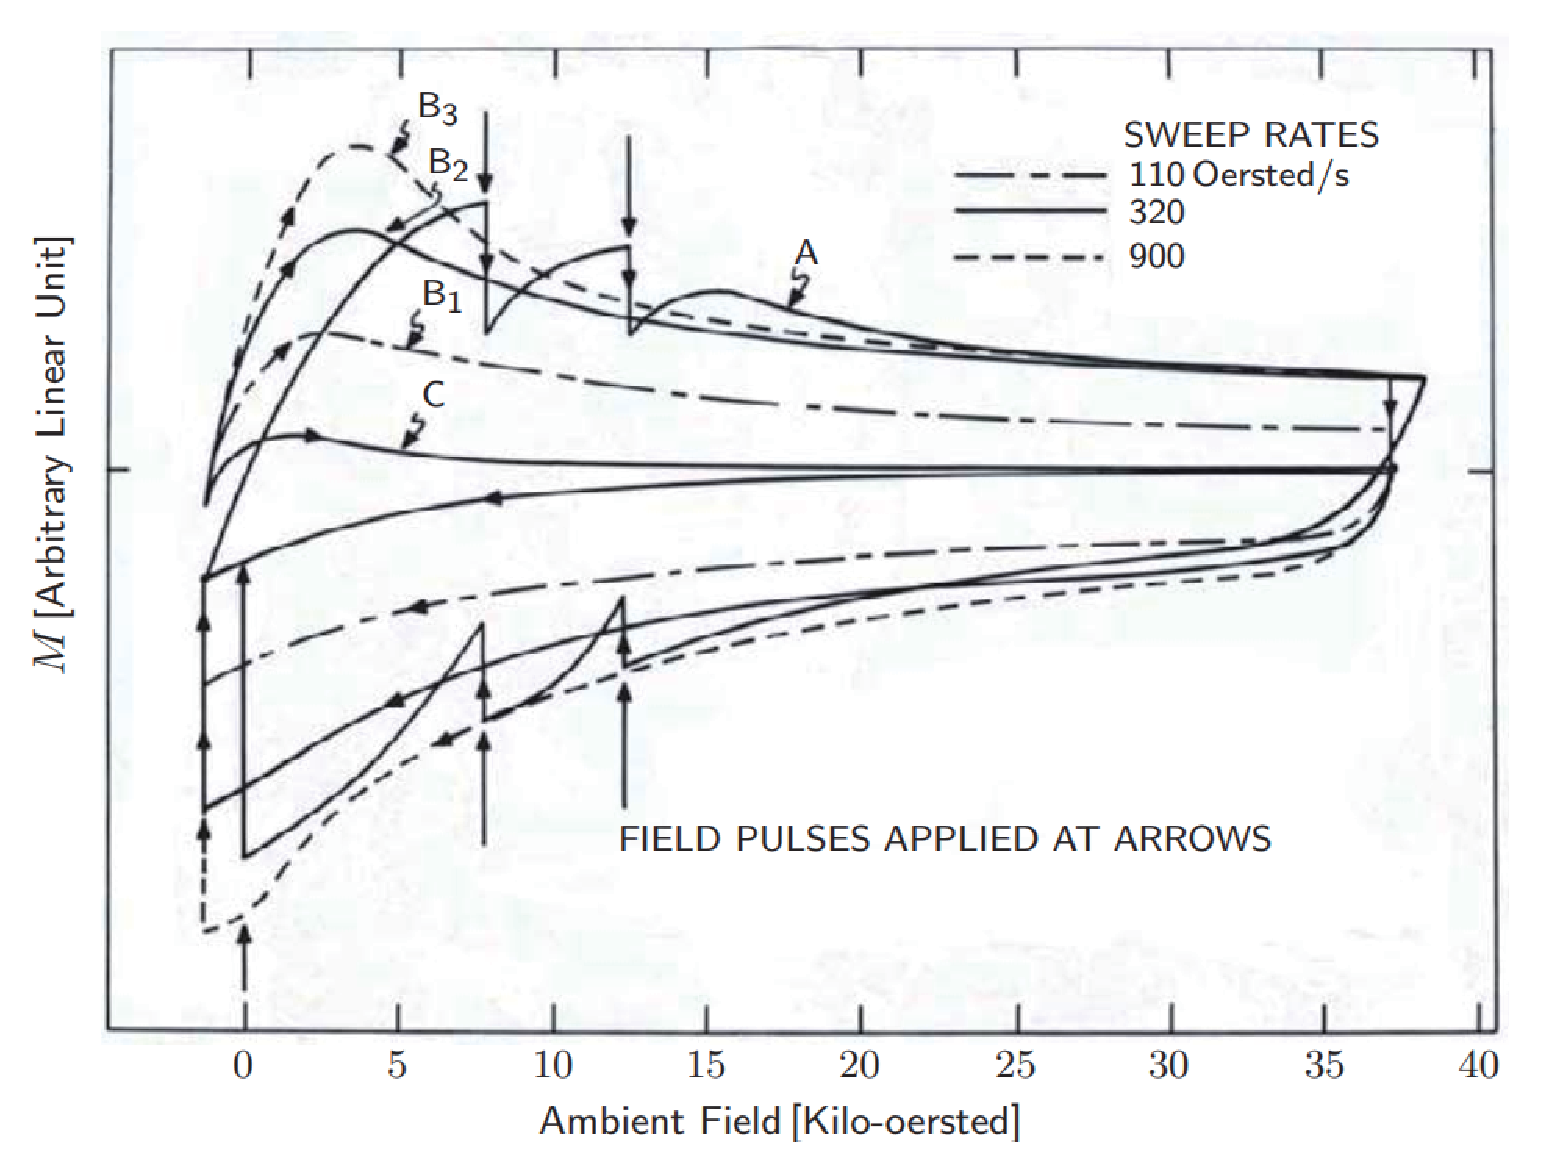
\includegraphics[scale=0.4]{chpt5/figs/fig5.21.eps}
	\caption{导体1,2,3的磁化迹线}
\end{figure}


\subsubsection{问题5.5之解}
a) Note that Traces A and C are independent of field sweep rate and that the
corresponding magnetization—an indication of filament diameter—is much greater
for Trace A than that for Trace C. We therefore conclude that Trace A is for
Conductor 3 (monofilament) and that Trace C is for Conductor 1 ($\ell_{p1}$). That
leaves Trace B for Conductor 2 ($\ell_{p2}$). (Remember that each conductor has the
same volume of NbTi superconductor, and thus its measured magnetization should
be directly proportional to filament diameter.)

b) The ratio of magnetization width, ($M(H_e\uparrow) − M(H_e\downarrow)$) of Conductor 3
(monofilament, Trace A) to that of Conductor 1 (Trace C), is roughly 10 for μ◦He
below ∼1T (10 kilo-oersted). Therefore, we conclude that the filament diameter
ratio is roughly 10.

c) Because a field sweep-rate of 900 oersted/sec ($\mu_0 \.{H}_{0z}$= 0.09 T/s) makes the
magnetization of Conductor 2 (Trace B3) nearly equal to that of Conductor 3
(Trace A), we may conclude that this sweep rate makes Conductor 2’s filament
twist pitch length$\ell_{p2}$critical. Thus from Eq. 5.44:
\begin{align*}%page348 第1个
\ell_{p2}=2\sqrt{\frac{2\rho_{cu}J_{c}d_{f}}{\mu_{o}\dot{H}_{0z}}} \tag{S5.1}
\end{align*}
代入$\rho_{cu}= 2\times 10^{−10}\ \mathrm{\Omega m}$%; Jcdf = 4×104 A/m; and μ◦ ˙H0z = 0.09 T/s, we obtain:
\begin{align*}%page348 第2个
\ell_{p2}&=2\sqrt{\frac{(2)(2\times 10^{10}\ \mathrm{\Omega m})(4\times 10^{4}\ \mathrm{A/m})}{0.09\ \mathrm{T/S}}}\\
&=2.7\times 10^{-2}\ \mathrm{m}=27\ \mathrm{mm}
\end{align*}
This value is close enough to the actual twist pitch of 10 mm. Because the magnetization
of Conductor 1 (Trace C) at a sweep rate of 320 oersted/sec is considerably
smaller than that of Conductor 2 for the same field sweep rate, we conclude that$\ell_{p1}$is significantly shorter than$\ell_{p2}$

\subsection{讨论5.6:换位}
An important implication of the condition Icp = Jcdf , used to derive Eq. 5.44
(PROBLEM 5.4), is that the two superconducting slabs are electrically coupled.
Were the conductor length substantially shorter than$2\ell_{c}$, on the other hand, the
two would be decoupled. In reality, these slabs may be decoupled, even if each one
is much longer than$2\ell_{c}$, if they are alternated in their positions with a pitch length
less than$2\ell_{c}$. In multifilamentary conductors, we can achieve partial decoupling
by twisting the wires with a pitch length$\ell_p\ll 2\ell_{c}$;$2\ell_{c}$must be small when$\.{H}_{0z}$is large. Note that in a twisted conductor each filament remains at a fixed radial
distance from the strand axis. By contrast, in a cable of transposed strands, more
complete decoupling is possible, because when strands are transposed each strand
is made to occupy every radial position across the cable diameter as it spirals along
the cable’s transposition length.


\subsection{讨论5.7:HTS中的磁通跳跃?}
\textbf{A. “完全”磁通跳跃的尺度判据}

The conductor size criterion (Eq. 5.40) was originally derived for LTS in the limit
$\Delta e_\phi/\Delta T=C_s$, where Cs is the superconductor heat capacity per unit volume,
assumed constant. Because in LTS, the temperature excursion in a complete flux
jump, i.e., Tc−Top, is small, this size criterion is adequate.

A general condition for suppression of flux jumping, under adiabatic conditions, is
that the superconductor’s magnetic energy must be less than its thermal density.
Under adiabatic conditions a flux jump can proceed to completion only if the
initial magnetic energy density at $T_{op}, e_\phi(T_{op})$, exceeds the thermal energy density
required to heat the superconductor from Top to Tc:
\begin{equation}%page349 5.45
e_{\phi}(T_{op})\geq h_{s}(T_{c})-h_{s}(T_{op})
\end{equation}
where hs(Tc) and hs(Top) are the superconductor enthalpies, respectively, at Tc and
Top. Because eφ(Top)=[μ◦Hp(Top)]2/6μ◦, and for Bean slab, Hp(Top)=aJc(Top),
the conductor size criterion, ac, for suppressing complete flux jumping is given by:
\begin{equation}%page349 第2个
a_{c}=\sqrt{\frac{6[h_{s}(T_{c})-h_{s}(T_{op})]}{\mu_{o}J_{c}^{2}(T_{op})}}
\end{equation}
Comparing these two size criteria (Eqs. 5.40 and 5.46), we may conclude that under
adiabatic conditions, a flux jump may initiate if the conductor size is greater than
that specified by Eq. 5.40, but it may be only “partial” if the size does not exceed
that of Eq. 5.46. Thus, flux jumps will be only partial in a superconductor that
either violates the size criterion of Eq. 5.40 but not Eq. 5.46, or the process is not
adiabatic. Note that even those flux jumps seen in Fig. 5.19 are, strictly speaking,
not complete, most probably because the process was not perfectly adiabatic.

\textbf{B. HTS中的磁通跳跃}

Because Tc is ∼100K in HTS, under adiabatic conditions the energy condition of
Eq. 5.45 is unlikely to be satisfied. Flux jumping is unlikely in HTS.

For YBCO with Top=77K and Tc=93K (zero field and current), for example, the
enthalpy difference is$\simeq$20MJ/m3 (60\% of the enthalpy difference for copper—
from Cp differences of the two materials at 120 K), and with Jc(Top)=1010 A/m2,
we compute, from Eq. 5.46: ac$\simeq$1mm (∼2mm diameter). Note that a YBCO
wire of 2-mm diameter will have a “Bean” magnetization, μ◦M=μ◦aJc(Top)∼2T.

Despite our expectation for HTS, flux jumps, not merely partial but also complete,
have been observed in HTS, for example, in “thin” crystals, 2a=4.2 mm,
with a y-axis extent of 0.2mm (thus “thin” rather than$\infty$as in a Bean slab) of
BSCCO-2212 [5.13] and thin (∼100-μm) films of Type II superconductors including
YBCO[5.14]. Nevertheless, in a real magnet-grade-superconductor, even of
HTS, because it must satisfy many requirements, including limiting AC losses, the
requirement that imposes, among other conditions, a severe size restriction, flux
jumping should be one of the least troubling aspects for HTS magnets.
